\documentclass[]{mcom-l}


\usepackage{latexsym,amsfonts,amsmath,amssymb,amsthm,epsfig,extdash,multirow}
\usepackage{stackrel,tabularx,mathtools,enumitem,longtable,xspace}
\usepackage[dvipsnames]{xcolor}
%\usepackage[numbers,sort&compress]{natbib}
\usepackage{hyperref,accents, booktabs}
\usepackage{algorithm, algorithmicx}
\usepackage{anyfontsize}
\usepackage{cleveref}
\usepackage{wrapfig}
\usepackage[font=small,labelfont=bf]{caption}

\usepackage{algpseudocode}
\usepackage{algorithm, algorithmicx}
\algnewcommand\algorithmicparam{\textbf{Parameters:}}
\algnewcommand\PARAM{\item[\algorithmicparam]}
\algnewcommand\algorithmicinput{\textbf{Input:}}
\algnewcommand\INPUT{\item[\algorithmicinput]}
\algnewcommand\RETURN{\State \textbf{Return }}
\usepackage{algpseudocode}

\theoremstyle{theorem}
\newtheorem{theorem}{Theorem}
\theoremstyle{remark}
\newtheorem{example}{Example}
%%list of acronyms with links
\newcommand{\QMCSoft}{QMCSoft\xspace}
\newcommand{\GAIL}{GAIL\xspace}
\newcommand{\QMC}{QMC\xspace}
\newcommand{\IIDMC}{IID MC\xspace}
\newcommand{\SAMSIQMC}{SAMSI-QMC\xspace}
\newcommand{\SciPy}{SciPy\xspace}
\newcommand{\GSL}{GSL\xspace}
\newcommand{\NAG}{NAG\xspace}
\newcommand{\MATLAB}{MATLAB\xspace}
\newcommand{\Chebfun}{Chebfun\xspace}
\newcommand{\Rlang}{R\xspace}
\newcommand{\Julia}{Julia\xspace}


%\textwidth6.5in
%\setlength{\oddsidemargin}{0in}
%\setlength{\evensidemargin}{0in}
%\textheight9.0in
%\textheight9.1in



\providecommand{\FJHickernell}{Hickernell}
\newcommand{\hf}{\widehat{f}}
\newcommand{\hg}{\widehat{g}}
\newcommand{\hI}{\hat{I}}
\newcommand{\hatf}{\hat{f}}
\newcommand{\hatg}{\hat{g}}
\newcommand{\tf}{\widetilde{f}}
\newcommand{\tbf}{\tilde{\bff}}
\newcommand{\vBall}{\text{vBall}_n}
\newcommand{\vEll}{\text{vEll}}

% Math operators
\DeclareMathOperator{\GP}{\mathcal{G} \! \mathcal{P}}
\DeclareMathOperator*{\argmax}{arg\,max}
\DeclareMathOperator*{\argmin}{arg\,min}
\DeclareMathOperator{\ALG}{ALG}
\DeclareMathOperator{\ACQ}{ACQ}
\DeclareMathOperator{\ERR}{ERR}
\DeclareMathOperator{\Prob}{\mathbb{P}}
\DeclareMathOperator{\diag}{diag}
\DeclareMathOperator{\vol}{vol}
\DeclareMathOperator{\errP}{ERRP}
\DeclareMathOperator{\errK}{ERRK}
\DeclareMathOperator{\errBd}{ERRBD}
\DeclareMathOperator{\APP}{APP}
\DeclareMathOperator{\Ex}{\mathbb{E}}
\newcommand{\TREND}{\textup{T}}
\newcommand{\VAR}{\textup{V}}
\newcommand{\LS}{\textup{LS}}

\newcommand{\NT}{{N_{\mT}}}
\newcommand{\Ntheta}{{N_{\btheta}}}


\newcommand{\reals}{{\mathbb{R}}}
\newcommand{\naturals}{{\mathbb{N}}}
\newcommand{\natzero}{{\mathbb{N}_0}}
\newcommand{\integers}{{\mathbb{Z}}}
\def\expect{{\mathbb{E}}}
\def\il{\left \langle}
\def\ir{\right \rangle}
\def\e{\varepsilon}
\def\g{\gamma}
\def\l{\lambda}
\def\b{\beta}
\def\a{\alpha}
\def\lall{\Lambda^{{\rm all}}}
\def\lstd{\Lambda^{{\rm std}}}

\newcommand{\vf}{\boldsymbol{f}}
\newcommand{\hV}{\widehat{V}}
\newcommand{\tV}{\widetilde{V}}
\newcommand{\fraku}{\mathfrak{u}}
\newcommand{\hcut}{\mathfrak{h}}
\newcommand{\tOmega}{\widetilde{\Omega}}
\newcommand{\tvarrho}{\widetilde{\varrho}}

\newcommand{\bbE}{\mathbb{E}}
\newcommand{\tQ}{\widetilde{Q}}
\newcommand{\mA}{\mathsf{A}}
\newcommand{\mB}{\mathsf{B}}
\newcommand{\mC}{\mathsf{C}}
\newcommand{\mD}{\mathsf{D}}
\newcommand{\mG}{\mathsf{G}}
\newcommand{\mH}{\mathsf{H}}
\newcommand{\mI}{\mathsf{I}}
\newcommand{\bbK}{\mathbb{K}}
\newcommand{\mK}{\mathsf{K}}
\newcommand{\tmK}{\widetilde{\mathsf{K}}}
\newcommand{\mL}{\mathsf{L}}
\newcommand{\mM}{\mathsf{M}}
\newcommand{\mP}{\mathsf{P}}
\newcommand{\mQ}{\mathsf{Q}}
\newcommand{\mR}{\mathsf{R}}
\newcommand{\mT}{\mathsf{T}}
\newcommand{\mU}{\mathsf{U}}
\newcommand{\mX}{\mathsf{X}}
\newcommand{\mZero}{\mathsf{0}}
\newcommand{\mPhi}{\mathsf{\Phi}}
\newcommand{\mPsi}{\mathsf{\Psi}}
\newcommand{\mLambda}{\mathsf{\Lambda}}
\newcommand{\cube}{[0,1]^d}
\newcommand{\design}{\{\bx_i\}_{i=1}^n}




\newcommand{\bone}{\boldsymbol{1}}
\newcommand{\bzero}{\boldsymbol{0}}
\newcommand{\binf}{\boldsymbol{\infty}}
\newcommand{\ba}{{\boldsymbol{a}}}
\newcommand{\bb}{{\boldsymbol{b}}}
\newcommand{\bc}{{\boldsymbol{c}}}
\newcommand{\bd}{{\boldsymbol{d}}}
\newcommand{\be}{{\boldsymbol{e}}}
\newcommand{\bff}{{\boldsymbol{f}}}
\newcommand{\bhh}{{\boldsymbol{h}}}
\newcommand{\beps}{{\boldsymbol{\varepsilon}}}
\newcommand{\tbeps}{\tilde{\beps}}
\newcommand{\bx}{{\boldsymbol{x}}}
\newcommand{\bX}{{\boldsymbol{X}}}
\newcommand{\bh}{{\boldsymbol{h}}}
\newcommand{\bj}{{\boldsymbol{j}}}
\newcommand{\bk}{{\boldsymbol{k}}}
\newcommand{\vell}{{\boldsymbol{\ell}}}
\newcommand{\bL}{{\boldsymbol{L}}}
\newcommand{\bg}{{\boldsymbol{g}}}
\newcommand{\bn}{{\boldsymbol{n}}}
\newcommand{\bp}{{\boldsymbol{p}}}
\newcommand{\bP}{{\boldsymbol{P}}}
\newcommand{\br}{{\boldsymbol{r}}}
\newcommand{\bv}{{\boldsymbol{v}}}
\newcommand{\bu}{{\boldsymbol{u}}}
\newcommand{\by}{{\boldsymbol{y}}}
\newcommand{\bt}{{\boldsymbol{t}}}
\newcommand{\bU}{{\boldsymbol{U}}}
\newcommand{\bz}{{\boldsymbol{z}}}
\newcommand{\bvarphi}{{\boldsymbol{\varphi}}}
\newcommand{\bgamma}{{\boldsymbol{\gamma}}}
\newcommand{\bdelta}{{\boldsymbol{\delta}}}
\newcommand{\bDelta}{{\boldsymbol{\Delta}}}
\newcommand{\bphi}{{\boldsymbol{\phi}}}
\newcommand{\bpsi}{{\boldsymbol{\psi}}}
\newcommand{\btheta}{{\boldsymbol{\theta}}}
\newcommand{\bnu}{{\boldsymbol{\nu}}}
\newcommand{\balpha}{{\boldsymbol{\alpha}}}
\newcommand{\bbeta}{{\boldsymbol{\beta}}}
\newcommand{\bo}{{\boldsymbol{\omega}}}  %GF added
\newcommand{\newton}[2]{\left(\begin{array}{c} #1\\ #2\end{array}\right)}
\newcommand{\anor}[2]{\| #1\|_{\mu_{#2}}}
\newcommand{\satop}[2]{\stackrel{\scriptstyle{#1}}{\scriptstyle{#2}}}
\newcommand{\setu}{{\mathfrak{u}}}

\newcommand{\me}{\textup{e}}
\newcommand{\mi}{\textup{i}}
\def\d{\textup{d}}
\def\dif{\textup{d}}
\newcommand{\cc}{\mathcal{C}}
\newcommand{\cb}{\mathcal{B}}
\newcommand{\cl}{L}
\newcommand{\ct}{\mathfrak{T}}
\newcommand{\cx}{{\Omega}}
\newcommand{\cala}{{\mathcal{A}}}
\newcommand{\calc}{{\mathcal{C}}}
\newcommand{\calf}{{\mathcal{F}}}
\newcommand{\calfd}{{\calf_d}}
\newcommand{\calh}{{\mathcal{H}}}
\newcommand{\tcalh}{{\widetilde{\calh}}}
\newcommand{\calI}{{\mathcal{I}}}
\newcommand{\calhk}{\calh_d(K)}
\newcommand{\calg}{{\mathcal{G}}}
\newcommand{\calgd}{{\calg_d}}
\newcommand{\caln}{{\mathcal{N}}}
\newcommand{\calp}{{\mathcal{P}}}
\newcommand{\cals}{{\mathcal{S}}}
\newcommand{\cL}{\mathcal{L}}
\newcommand{\cP}{\mathcal{P}}
\newcommand{\cT}{\mathcal{T}}
\newcommand{\cK}{\mathcal{K}}
\newcommand{\fA}{\mathfrak{A}}
\newcommand{\fC}{\mathfrak{C}}
\newcommand{\fF}{\mathfrak{F}}
\newcommand{\fL}{\mathfrak{L}}
\newcommand{\fU}{\mathfrak{U}}
\newcommand{\hS}{\widehat{S}}

\def\abs#1{\ensuremath{\left \lvert #1 \right \rvert}}
\newcommand{\bigabs}[1]{\ensuremath{\bigl \lvert #1 \bigr \rvert}}
\newcommand{\norm}[2][{}]{\ensuremath{\left \lVert #2 \right \rVert}_{#1}}
\newcommand{\ip}[3][{}]{\ensuremath{\left \langle #2, #3 \right \rangle_{#1}}}
\newcommand{\bignorm}[2][{}]{\ensuremath{\bigl \lVert #2 \bigr \rVert}_{#1}}
\newcommand{\Bignorm}[2][{}]{\ensuremath{\Bigl \lVert #2 \Bigr \rVert}_{#1}}
\newcommand{\calm}{{\mathfrak{M}}}

\newcommand{\des}{\{\bx_i\}}
\newcommand{\desinf}{\{\bx_i\}_{i=1}^{\infty}}
\newcommand{\desn}{\{\bx_i\}_{i=1}^n}
\newcommand{\wts}{\{g_i\}_{i=1}^N}
\newcommand{\wtsn}{\{g_i\}_{i=1}^N}
\newcommand{\datan}{\{y_i\}_{i=1}^N}

%FJH added
\newcommand{\Order}{\mathcal{O}}
\newcommand{\ch}{\mathcal{H}}
\newcommand{\tch}{{\widetilde{\ch}}}
\newcommand{\veps}{\boldsymbol{\varepsilon}}
\DeclareMathOperator{\best}{best}
\newcommand{\hmu}{\hat{\mu}}
\newcommand{\hsigma}{\hat{\sigma}}
\newcommand{\tK}{\widetilde{K}}
%\newcommand{\Matlab}{{\sc Matlab}\xspace}
\newcommand{\abstol}{\varepsilon_{\text{a}}}
\newcommand{\reltol}{\varepsilon_{\text{r}}}

\newcommand\starred[1]{\accentset{\star}{#1}}

\newcommand{\designInf}{\{\bx_i\}_{i=1}^\infty}
\newcommand{\dataN}{\bigl\{\bigl(\bx_i,f(\bx_i)\bigr)\bigr\}_{i=1}^n}
\newcommand{\dataNp}{\bigl\{\bigl(\bx_i,f(\bx_i)\bigr)\bigr\}_{i=1}^{n'}}
\newcommand{\dataNo}{\bigl\{\bigl(\bx_i,f(\bx_i)\bigr)\bigr\}_{i=1}^{n_0}}
\newcommand{\ErrN}{\ERR\bigl(\dataN,n\bigr)}
\newcommand{\fint}{f_{\text{int}}}
\newcommand{\inflate}{\fC}
\DeclareMathOperator{\spanV}{span}

\newcommand{\FredNote}[1]{{\color{blue}Fred: #1}}
\newcommand{\YuhanNote}[1]{{\color{magenta}Yuhan: #1}}

\title[Adaptive Multivariate Function Approximation]{Adaptive Multivariate Function Approximation for Cones of Functions via Minimum Hilbert Space Norm Interpolants}
\author{Yuhan Ding}

\author{Fred J. Hickernell}
\address{RE 220, Department of Applied Mathematics, Illinois Institute of Technology, Chicago, IL 60616}
\email{hickernell@iit.edu}
\date{\today}

\begin{document}

\maketitle

\section{Introduction}
Rigorous error bounds for numerical approximations typically consist of the norm of the input function multiplied by the norm of the error operator.  Because the norm of the input function is unknown, these error bounds cannot tell us whether a prescribed error tolerance has been met.  Adaptive numerical algorithms typically use heuristic, data-driven error bounds,  so we don't know when they can be trusted.

We propose  adaptive function approximation algorithms based on rigorous, data-driven error bounds.  Each algorithm assumes that the function to be approximated lies in a \emph{candidate cone}, $\cc$.  ``Candidate'' means functions that our algorithm can approximate accurately.  The definition of $\cc$ formalizes the idea that \emph{what we observe is nearly what we get}.  If $f$ lies in $\cc$, then any constant multiple of $f$  also lies in $\cc$, which makes $\cc$ a cone.  Although there are no data-driven \emph{sufficient} conditions for a function lie in $\calc$, there are necessary conditions.

Our underlying numerical approximation is the reproducing kernel Hilbert space (RKHS) minimum norm interpolant with an explicit error bound.  Baking into $\cc$ the assumption that the norm of a function is not arbitrarily larger than the norm of its interpolant allows us to construct a rigorous adaptive function approximation algorithm. Given a black-box input function, $f$, and an error tolerance, $\varepsilon$, our algorithm returns an approximation, $\ALG(f,\varepsilon) \in L^\infty$---defined only in terms of function values---for which 
\begin{equation} \label{eq:errorcrit}
\norm[\infty]{f - \ALG(f,\varepsilon)} \le \varepsilon \qquad \forall f\in \cc.
\end{equation}

Adaption can take several forms, including
\begin{itemize}
    \item Adaptive choice of the number of function data needed, $n$, (Section \ref{sec:basicIdea} and Algorithm \ref{alg:basicadapt}),
    \item Adaptive choice of the data sites, $\{\bx_1, \bx_2, \ldots\}$,  (Section \ref{sec:adaptSites} and Algorithm \ref{alg:adaptsample}), and
    \item Adaptive choice of the function space, $\calf$, for which the input function is typical  (Section \ref{sec:adaptF} and Algorithm \ref{alg:adapttheta}).
\end{itemize}
Our theory develops progressively by adding additional forms of adaption for functions lying purely in a RKHS and constructing increasingly sophisticated algorithms.  In Section \ref{sec:poly} and Algorithm \ref{alg:trend} we generalize to the setting where a finite dimensional space of possible trends---e.g., polynomials of fixed degree---are exactly reproduced.

These algorithms draw upon the well-developed literature of RKHS function approximation \cite{Buh03a,Fas07a,FasMcC15a,ForFly15a,ForEtal09,RasWil06a,SchWen06a,Wah85a,Wen05a}.  Our main contributions are 
\begin{itemize}
	\item The candidate cone (Section \ref{sec:basicIdea}),
	\item A geometric interpretation of the data-based inference of a suitable RKHS (Section  \ref{sec:adaptTheta}), and
	\item Inferring the location dependence of the reproducing kernel (Section \ref{sec:InferSpace}).
\end{itemize}

Any algorithm that claims to satisfy \eqref{eq:errorcrit} cannot possibly do so for $\cc$ corresponding to an infinite dimensional vector space.  If there were such an algorithm, then $\ALG(0,\varepsilon)$ would terminate after evaluating the zero function at some data sites $\bx_1, \ldots, \bx_n$ for some positive integer $n$.  Since $\cc$ is infinite dimensional, there exists some $g \in \cc$, for which $g(\bx_1) = \cdots = g(\bx_n) = 0$ but for which $\norm[\infty]{g} > 2 \varepsilon$.  That is, $g$ looks like  $0$ to the algorithm, $\ALG(g,\varepsilon) = \ALG(0,\varepsilon)$, but is not close enough to $0$.   Since $\ALG(0,\varepsilon)$ cannot be within distance $\varepsilon$ of both the zero function and $g$, error criterion \eqref{eq:errorcrit} is not satisfied.

Function approximation algorithms are often constructed to satisfy error criterion \eqref{eq:errorcrit} for a candidate \emph{ball}, e.g., $\cc = \{f \in \calf : \norm[\calf]{f} \le 1\}$.  Choosing this convex, symmetric candidate set guarantees that adaption is of no value \cite{Bak71}.  Here, we choose candidate cones that are unbounded and non-convex, which makes them amenable to adaptive algorithms.

The algorithms constructed here put a premium on the cost of obtaining function values.  We have in mind the situation where one function value may be the output of an expensive simulation requiring hours or days, denoted $\$(f)$.  Our algorithm produces an inexpensive surrogate or approximation of the expensive simulation.  If $n$ function values are required to obtain a satisfactory function approximation, then we do not mind if manipulating that data to construct our function approximation requires $\Order(n^p)$ operations, since practically speaking this will be smaller than $\$(f) n$.  RKHS minimum  norm interpolants typically require $\Order(n^3)$ operations, and we may require more operations to tune the kernel and obtain a satisfactory error bound.  Methods to reduce the computational effort required to construct RKHS minimum norm interpolants include an estimating equation approach \cite{AniCheSte16a}, approximation by incomplete Cholesky factorizations \cite{OwhEtal19a}, and matching designs with kernels to obtain Gram matrices that can be inverted using fast transforms \cite{RatHic19a}.


%%%%%%%%%%%%%%%%%%%%%%%%%%%%%%%%%%%%%%%%%%%%%%%%%%%%%%%%%%%%%%%%%%%%%%
%%%%%%%%%%%%%%%%%%%%%%%%%%%%%%%%%%%%%%%%%%%%%%%%%%%%%%%%%%%%%%%%%%%%%%
\section{Adaptive Function Approximation for a Fixed Hilbert Space} \label{sec:fixedF}
%%%%%%%%%%%%%%%%%%%%%%%%%%%%%%%%%%%%%%%%%%%%%%%%%%%%%%%%%%%%%%%%%%%%%%
%%%%%%%%%%%%%%%%%%%%%%%%%%%%%%%%%%%%%%%%%%%%%%%%%%%%%%%%%%%%%%%%%%%%%%

%%%%%%%%%%%%%%%%%%%%%%%%%%%%%%%%%%%%%%%%%%%%%%%%%%%%%%%%%%%%%%%%%%%%%%
%%%%%%%%%%%%%%%%%%%%%%%%%%%%%%%%%%%%%%%%%%%%%%%%%%%%%%%%%%%%%%%%%%%%%%
\subsection{The Basic Idea Our Adaptive Algorithm} \label{sec:basicIdea}
%%%%%%%%%%%%%%%%%%%%%%%%%%%%%%%%%%%%%%%%%%%%%%%%%%%%%%%%%%%%%%%%%%%%%%
%%%%%%%%%%%%%%%%%%%%%%%%%%%%%%%%%%%%%%%%%%%%%%%%%%%%%%%%%%%%%%%%%%%%%%
Suppose that $f$ belongs to an RKHS $\calf$ of functions with domain $\cx$.  Let $K: \Omega \times \Omega \to \reals$ denote the reproducing kernel.  Let $\mX = (\bx_1, \ldots, \bx_n)^T \in \cx^n \subseteq \reals^{n \times d}$ be an array of $n$ data sites, and let $\by  = f(\mX) \in \reals^n$ denote the array of function values at these data sites.  
The minimum $\calf$-norm interpolant of $f$ is 
\begin{subequations} \label{eq:RKHSAPP}
\begin{align} 
\APP(\mX,\by) &= \sum_{i=1}^n c_i K(\bx_i,\cdot) = \bc^T K(\mX,\cdot) =  K(\cdot, \mX) \mK^{-1} \by, \\
 \text{where } & \qquad \bc = \mK^{-1} \by, \quad \mK = K(\mX,\mX) = \bigl( K(\bx_i,\bx_j) \bigr)_{i,j=1}^n,  \\
& \qquad  K(\mX,\bx) = \bigl(K(\bx,\bx_i) \bigr)_{i=1}^n =  K(\bx, \mX)^T.
\end{align}
\end{subequations}
This approximation lies in the $n$-dimensional subspace $\calf_{\mX} := \{\bc^T K(\mX,\cdot) : \bc \in \reals^n \}$, and the error of the approximation lies in the orthogonal infinite dimensional subspace $\calf_{\mX \perp} := \{g \in \calf : g(\mX) = \bzero\}$.
The approximation has a known pointwise error bound of \cite{bibid}:
\begin{subequations} \label{eq:RKHSErrBd}
\begin{align}
\abs{f(\bx) - \APP(\mX,\by)(\bx)} & \le  \errK(\mX,\bx) \, \bignorm[\calf]{f - \APP(\mX,\by)}  \qquad \forall f \in \calf,  \\
\text{where} & \errK(\mX,\bx) : = \sqrt{K(\bx,\bx) - K(\bx,\mX) \mK^{-1} K(\mX,\bx)}.
\end{align}
\end{subequations}
Here, $\errK(\mX,\bx)$ is the norm of the error functional $f \mapsto f(\bx)-\APP(\mX,f(\mX))(\bx)$.  It is also represents $\max \{\abs{g(\bx)} : g \in \calf_{\mX \perp}, \ \norm[\calf]{g} \le 1\}$.

\begin{figure}[H]
	\centering
	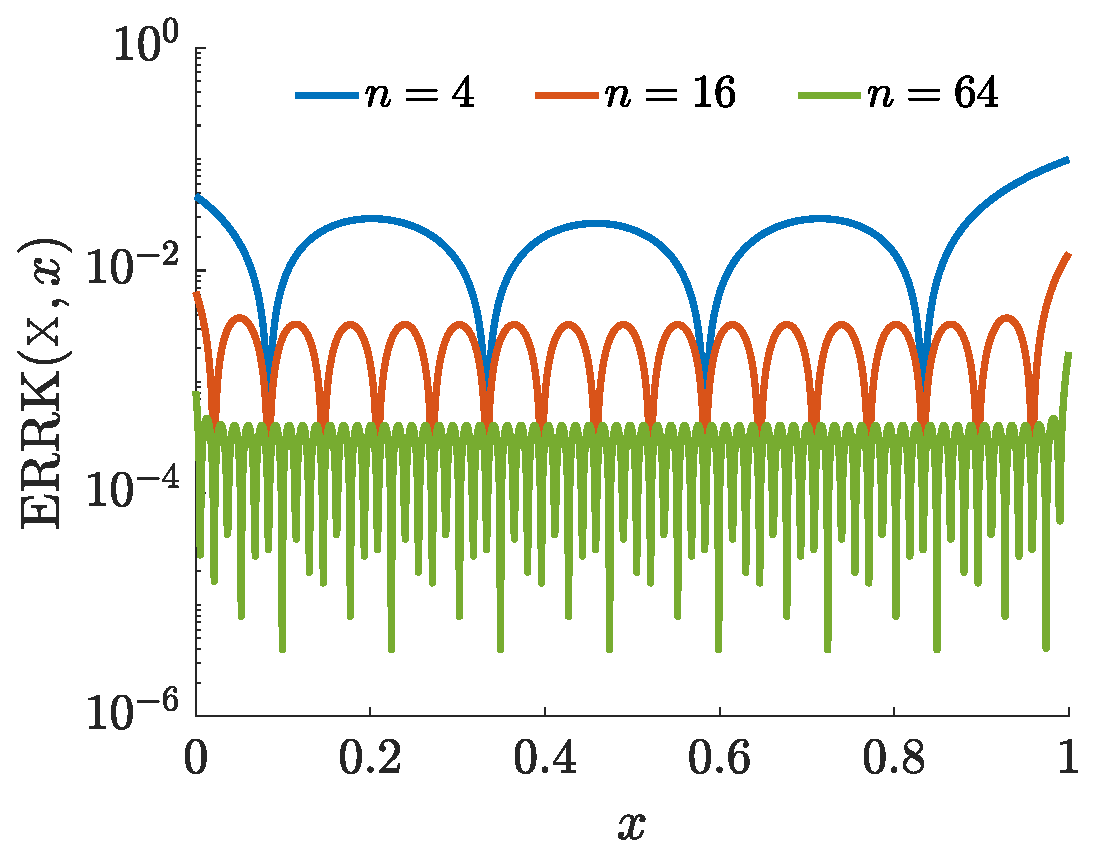
\includegraphics[height =6cm]{ProgramsImages/errKplot.eps}
	\caption{Plot of $\errK(\mX,\cdot)$ for various sample sizes.  The magnitude decreases in size as $n$ increases; $\errK(\mX,\bx) = 0$, when $\bx$ is a data site. \label{fig:errK}}
\end{figure}

Figure \ref{fig:errK} displays   $\errK(\mX,\cdot)$  for a reproducing kernel from the Mat\'ern family: 
	\begin{equation} \label{eq:MaternOne}
K(\bt,\bx) = (1 +  \norm{\bt-\bx}) \exp(-\norm{\bt-\bx}),
\end{equation}
where $\norm{\cdot}$ denotes the Euclidean norm.  The space-filling sequence of data sites is 
\begin{equation} \label{eq:FixedVDCDes}
\begin{array}{rccccccccc}
i  & 1 & 2 & 3 & 4 & 5 & 6 & 7 & 8 & \cdots\\
\midrule
x_i & 1/3 & 5/6 & 7/12 & 1/12 & 11/24 & 23/24 & 17/24 & 5 /24 & \cdots
\end{array}
\end{equation}
which is a van der Corput sequence \cite{} shifted by $1/3$ modulo one.  By definition, $\errK(\mX,\cdot)$ vanishes at the data sites.  Moreover, increasing the number of data sites decreases the magnitude of $\errK(\mX,\cdot)$, which likewise decreases the error bound in \eqref{eq:RKHSErrBd}.


Data-based approximation $\APP(\mX,\by)$ in \eqref{eq:RKHSAPP} is an ingredient in our adaptive algorithm, but error bound \eqref{eq:RKHSErrBd} contains the unknown factor $\norm[\calf]{f - \APP(\mX,\by)}$, which cannot be computed from function data.  We can compute  $\bignorm[\calf]{\APP(f)} = \sqrt{\by^T \mK^{-1} \by}$ from data using vector-matrix operations.  Moreover, since the error is orthogonal to the approximation,  the Pythagorean Theorem implies that $\norm[\calf]{f}^2  = \bignorm[\calf]{\APP(f)}^2 + \bignorm[\calf]{f - \APP(f)}^2$.  To establish a data-driven error bound, we define this candidate cone as follows:
\begin{align} \label{eq:RKHScone}
\calc &:= \Bigl\{f \in \calf : \norm[\calf]{f}^2 \le (1 + A^2(\mX)) \bignorm[\calf]{\APP(\mX,\by)}^2 \quad \forall \mX \in \Omega^d, \ \by = f(\mX) \Bigr \} \\
\nonumber
& = \Bigl \{f \in \calf : \bignorm[\calf]{f - \APP(f)} \le A(\mX) \bignorm[\calf]{\APP(\mX,\by)} \quad \forall \mX \in \Omega^d, \ \by = f(\mX) \Bigr \} \\
\nonumber
& = \Bigl \{f \in \calf : \bignorm[\calf]{f - \APP(f)}^2 \le \frac{A^2(\mX)}{1 + A^2(\mX)} \bignorm[\calf]{f}^2 \quad \forall \mX \in \Omega^d, \ \by = f(\mX) \Bigr \},
\end{align}
where $A(\cdot)$ is positive and fixed in advance.  A larger $A(\mX)$ implies a more inclusive candidate cone.  This $\calc$ is a cone because $f \in \calc$ implies $c f \in \calc$ for any real $c$. 

Our candidate cone is inspired by the intuition \emph{what we have not yet seen is not much worse than what we have seen}. All adaptive algorithms are based on this idea. Definition \eqref{eq:RKHScone} formalizes it. 

Because $\bignorm[\calf]{\APP(\mX,\by)} = \sqrt{\by^T \mK^{-1} \by}$, error bound \eqref{eq:RKHSErrBd} implies an error bound that can be computed solely based on the function data: 
\begin{subequations} \label{eq:DataErrBd}
\begin{align}
\label{eq:DataErrBdA}
    \MoveEqLeft\abs{f(\bx) - \APP(\mX,\by)(\bx)} \\
    \nonumber
    & \le   A(\mX) \errK(\mX,\bx) \sqrt{\by^T \mK^{-1} \by } =: \errBd(\mX,\by,\bx) \qquad \forall f \in \calc, \\
    \label{eq:DataErrBdB}
    \MoveEqLeft\norm[\infty]{f - \APP(\mX,\by)} \\ 
    \nonumber 
    & \le   A(\mX) \errK(\mX) \sqrt{\by^T \mK^{-1} \by } =: \errBd(\mX,\by) \qquad \forall f \in \calc, \\
    \text{where }& \qquad \errK(\mX) := \norm[\infty]{\errK(\mX,\cdot)}.
\end{align}
\end{subequations}
Here $\errK(\mX)$ represents the norm of the error operator $f \mapsto f-\APP(\mX,f(\mX))$.  It is also the represents $\max \{\norm[\infty]{g} : g \in \calf_{\mX \perp}, \ \norm[\calf]{g} \le 1\}$


This data-based error bound provides what  our adaptive algorithm needs.  Note that $n$ is implicit in the definition of the array of data sites, $\mX$, but we hide this dependence for notational simplicity.

\begin{algorithm}[H]
\caption{Adaptive Sample Size \label{alg:basicadapt}}
	\begin{algorithmic}
	\PARAM the RKHS, $\calf$; the factor, $A(\cdot)$, which defines  the candidate cone, $\cc$, in \eqref{eq:RKHScone};  a sequence of data sites, $\{\bx_1, \bx_2, \ldots \}$; an initial sample size, $n_0$
	\INPUT a black-box function, $f \in \cc$; an absolute error tolerance, $\varepsilon>0$

    \Ensure Error criterion $\norm[\infty]{f - \ALG(f,\varepsilon)} \le \varepsilon$

   \State Let $n \leftarrow n_0 -1$

\Repeat

\State Let $n \leftarrow n + 1$

\State Compute $\by$, $A(\mX)$, $K(\mX,\mX)$, and $K(\mX,\cdot)$

\Until $\errBd(\mX,\by) \le \varepsilon$

\RETURN $\ALG(f,\varepsilon) = \by^T \mK^{-1} K(\mX,\cdot)$

\end{algorithmic}
\end{algorithm}

This algorithm adaptively chooses the sample size so that the error criterion must be satisfied for all functions in the candidate cone $\cc$.  For a well chosen design, $\errK(\mX)$ tends to zero as $n$ increases.  A larger function yields larger function data $\by$, which implies that a larger sample size will be required to achieve the error criterion.

This algorithm is deficient.  The choice of the design does not yet depend in on the function data.  There is no assurance that the RKHS specified by the choice of $K$ fits $f$.  There is also the matter of how to choose $A(\mX)$.  These matters are addressed in the following (sub-)sections.


%%%%%%%%%%%%%%%%%%%%%%%%%%%%%%%%%%%%%%%%%%%%%%%%%%%%%%%%%%%%%%%%%%%%%%
%%%%%%%%%%%%%%%%%%%%%%%%%%%%%%%%%%%%%%%%%%%%%%%%%%%%%%%%%%%%%%%%%%%%%%
\subsection{Choosing a Reasonable $A$?}
%%%%%%%%%%%%%%%%%%%%%%%%%%%%%%%%%%%%%%%%%%%%%%%%%%%%%%%%%%%%%%%%%%%%%%
%%%%%%%%%%%%%%%%%%%%%%%%%%%%%%%%%%%%%%%%%%%%%%%%%%%%%%%%%%%%%%%%%%%%%%

The candidate cone depends on the factor $A(\mX)$, which, according to \eqref{eq:RKHScone}, reflects how much larger one expects $\bignorm[\calf]{f  - \APP(\mX,\by)}$ might be than $\bignorm[\calf]{\APP(\mX,\by)}$ is.  It is natural for $A(\mX)$ to depend  on the quality of the design and the number of data sites.  One measure of  design quality  is 
\begin{equation} \label{eq:BX}
B(\mX) : = \frac{ \sup \{\norm[\infty]{g} :  \norm[\calf]{g}  \le 1 , \ g(\mX) = 0 \}   }  {\sup \{ \norm[\infty]{g}  : \norm[\calf]{g}  \le 1  \} }
=  \frac{\errK(\mX)}{\sqrt{\norm[\infty]{K(\cdot,\cdot)}}} \le 1.
\end{equation}
As the sample size increases using well-placed data, $B(\mX)$ tends to zero.  Moreover, $B(\mX)$ does not depend on the vertical scaling of the kernel, $K$.  That is, replacing $K$ by $cK$ for any positive $c$ leaves $B$ unchanged.

The choice of $A(\mX)$ is  a value judgment.  We propose
\begin{equation} \label{eq:an}
A(\mX): = \begin{cases} \displaystyle
\frac{A_\infty B_0}{B_0 - B(\mX)}, & B(\mX) < B_0, \\
\infty, & B(\mX) \ge B_0.
\end{cases}
\end{equation}
The parameter $A_\infty > 0$ represents the limiting value of $A(\mX)$ as the design tends to perfection.  The parameter $B_0$ represents the maximum value of $B(\mX)$ for which one is willing to infer a bound on $\bignorm[\calf]{f  - \APP(\mX,\by)}$ in terms of $\bignorm[\calf]{\APP(\mX,\by)}$.  Making $A_\infty$ larger or $B_0$ smaller makes the candidate cone, $\cc$ more inclusive.

The parameter $n_0$ in Algorithm \ref{alg:basicadapt} can be chosen as the minimum sample size for which $B(\mX) < B_0$.  This leaves only the two parameters $A_\infty$ and $B_0$ as requiring default values or user choices.  Adaptive algorithms always require such default values.  For example, Chebfun \cite{DriHalTre14a}, a popular MATLAB package that solves numerical problems by representing functions by their Chebyshev series, requires a default initial number of data sites.




%%%%%%%%%%%%%%%%%%%%%%%%%%%%%%%%%%%%%%%%%%%%%%%%%%%%%%%%%%%%%%%%%%%%%%
%%%%%%%%%%%%%%%%%%%%%%%%%%%%%%%%%%%%%%%%%%%%%%%%%%%%%%%%%%%%%%%%%%%%%%
\subsection{Optimization Problems} \label{sec:Optim}
%%%%%%%%%%%%%%%%%%%%%%%%%%%%%%%%%%%%%%%%%%%%%%%%%%%%%%%%%%%%%%%%%%%%%%
%%%%%%%%%%%%%%%%%%%%%%%%%%%%%%%%%%%%%%%%%%%%%%%%%%%%%%%%%%%%%%%%%%%%%%

Algorithm \ref{alg:basicadapt} requires numerical optimization to  
approximate the sup-norms that appear in via the data-based error bound in \eqref{eq:DataErrBdB} and the definition of $B(\mX)$ in \eqref{eq:BX}.  Finding the locations of optima is required below in \eqref{eq:nextsample} for adaptively choosing the next data site and in \eqref{eq:thetEB} in Section \ref{sec:adaptF} for adaptively choosing the correct kernel.  We do not r identify the best numerical optimization algorithms for these purposes but recognize this as a problem for further research.  

These optimization problems do not require high accuracy answers.  Underestimating $\errK(\mX)$
in  \eqref{eq:DataErrBdB} or  \eqref{eq:BX} by several percent does not lead to significant loss of accuracy or efficiency.  
In our numerical examples, we approximate this quantity by direct search:
\begin{equation} \label{eq:normappx}
\errK(\mX) \approx \norm[\infty]{\errK(\mX,\mT)},
\end{equation}
where $\mT := (\bt_1, \ldots, \bt_\NT)^T \in \cx^\NT$ is a fixed array of test points.

\begin{example}
	\label{ex:adpsamplesize}
	To illustrate our algorithm, we consider a sinusoidal function\cite{}
	\begin{equation}
	f: x \mapsto  \sin(2\pi(x-0.1)), \qquad x \in [0,1],
	\end{equation}
	which is plotted in Figure \ref{fig:ex1}.  We apply Algorithm \ref{alg:basicadapt} to this example using the sequence of data sites described in \eqref{eq:FixedVDCDes} and for a sequence of error tolerances with
	$n_0 = 1$.  We choose the Mat\'ern kernel in \eqref{eq:MaternOne},  $A_\infty = 1, B_0 = 0.05$, and $\mT = (0, 0.001, \ldots, 1)^T$.  This table summarizes our results.  the bottom row shows the percentage of points in $\mT$ for which the pointwise error bound is valid.
	
	\input{ProgramsImages/Alg1_OutCurrinSineFun_Matern.txt}
	
	
	\begin{figure}[H]
		\centering
		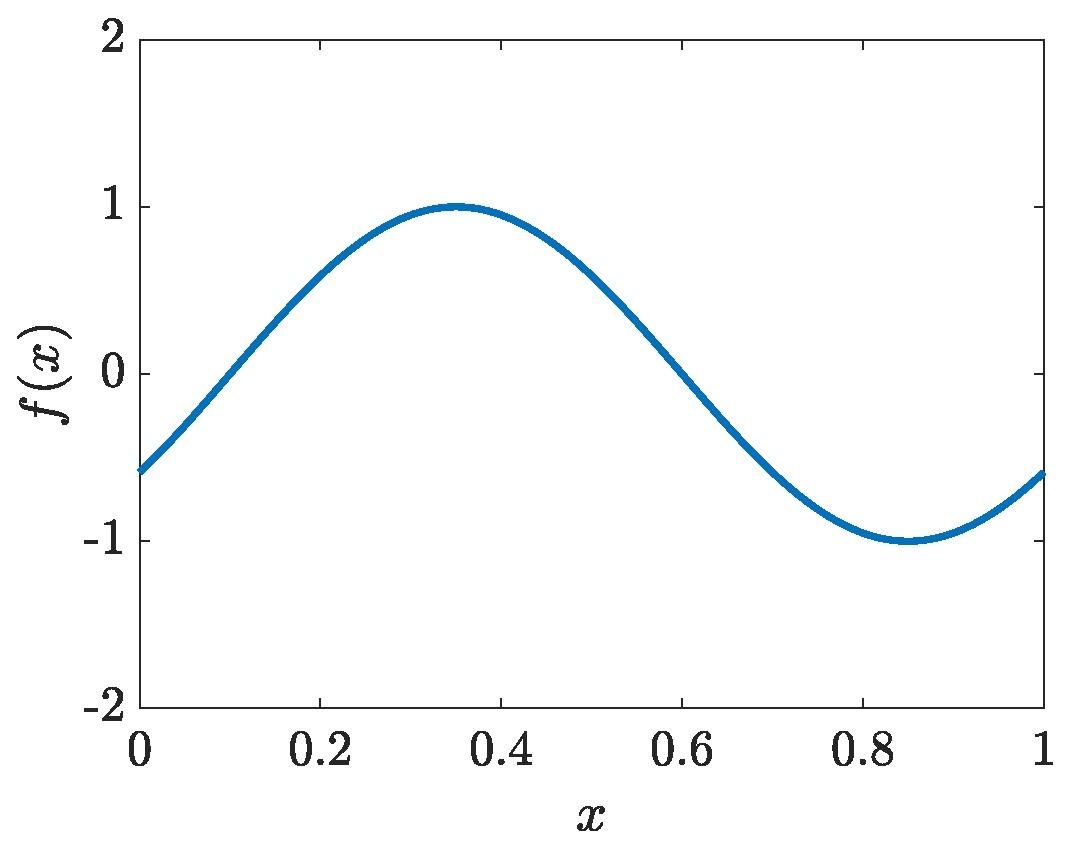
\includegraphics[height = 4.5cm]{ProgramsImages/CurrinSineFunPlot.eps} \qquad
		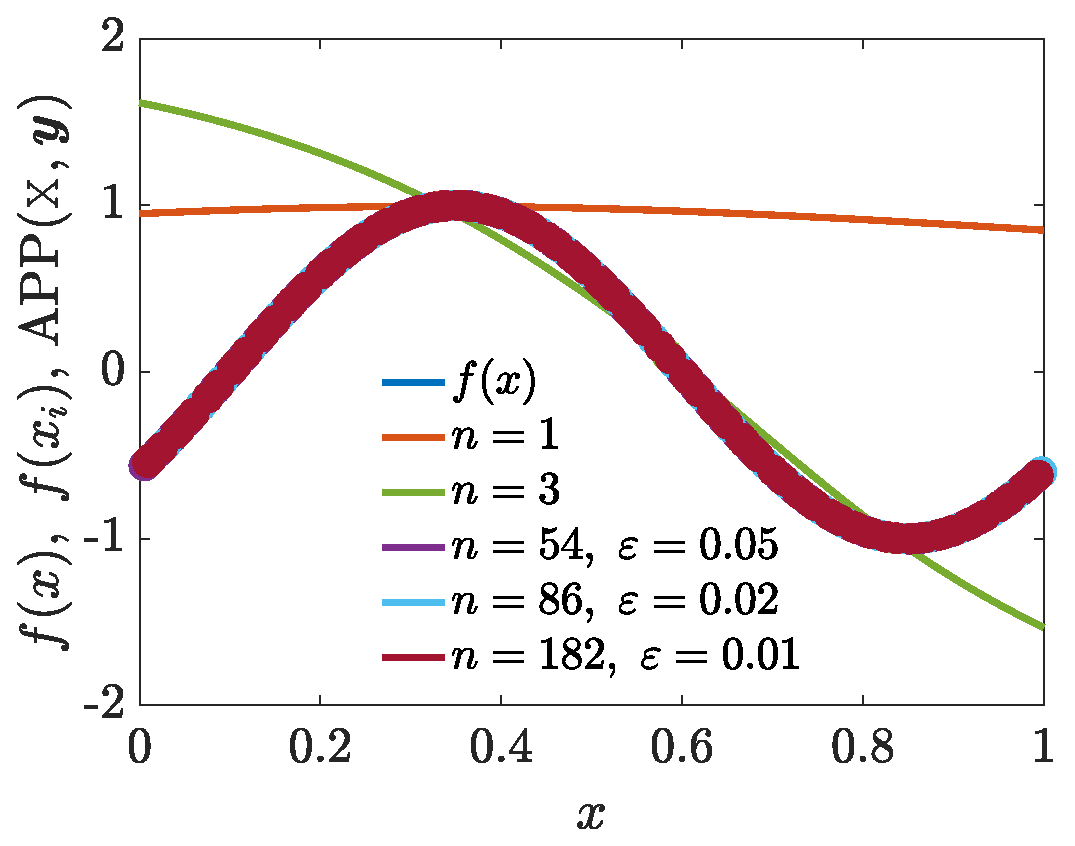
\includegraphics[height = 4.5cm]{ProgramsImages/Alg1_CurrinSineFun_Matern.eps}
		\caption{A plot of our example $f$ (left) and a plot of our RKHS minimum norm interpolant approximations for various $\varepsilon$ and  $n$ using Algorithm \ref{alg:basicadapt}.  Approximation improves as $n$ increases. \label{fig:ex1}}
	\end{figure}
	
Not suprisingly, the function approximation for $n=1$ is poor, but it improves as the sample size increases.  The true  maximum absolute error of the adaptive approximation does not exceed the data-driven error bound $\errBd(\mX,\by)$ for every tolerance selected here, and by design this error bound does not exceed the tolerance.  Moreover, the true pointwise error of the adaptive approximation does not exceed the pointwise error bound $\errBd(\mX,\by,\cdot)$ at any point $\mT$ for every tolerance selected here.  Moreover, for every $n$ up to $TBD$, the pointwise error bound holds for all points in  $\mT$.
	
\end{example} 

%%%%%%%%%%%%%%%%%%%%%%%%%%%%%%%%%%%%%%%%%%%%%%%%%%%%%%%%%%%%%%%%%%%%%%
%%%%%%%%%%%%%%%%%%%%%%%%%%%%%%%%%%%%%%%%%%%%%%%%%%%%%%%%%%%%%%%%%%%%%%
\subsection{Computational Cost} \label{sec:compCost}
%%%%%%%%%%%%%%%%%%%%%%%%%%%%%%%%%%%%%%%%%%%%%%%%%%%%%%%%%%%%%%%%%%%%%%
%%%%%%%%%%%%%%%%%%%%%%%%%%%%%%%%%%%%%%%%%%%%%%%%%%%%%%%%%%%%%%%%%%%%%%
We noted in the introduction that we are primarily concerned with the computational cost of obtaining function data, but we do count the cost of our algorithms.  The sequence of data vectors, $\by_1, \ldots, \by_n$, costs $\$(f)n$, explicitly showing that the cost of a function value might be quite large.  The Cholesky decompositions of $\mK_1, \ldots, \mK_n$ and $\mK_1^{-1}, \ldots, \mK_n^{-1}$ can all be computed in $\Order(n^3)$ operations using clever updating.  The quantity on the right side of \eqref{eq:normappx} can be computed recursively for $1, \ldots, n$ data sites using a total of $\Order\bigl( \NT n^2 \bigr)$ operations as well.  

Thus, the computational cost of Algorithm \ref{alg:basicadapt} is
\begin{equation} \label{eq:compcostbasic}
\Order\bigl(\$(f)n + n^3 + \NT n^2 \bigr),
\end{equation}
where $n$ is the final number of data sites required.  Again, our intended application is that for which $\$(f)$ dominates $n^2$ and $\NT n$.  



%%%%%%%%%%%%%%%%%%%%%%%%%%%%%%%%%%%%%%%%%%%%%%%%%%%%%%%%%%%%%%%%%%%%%%
%%%%%%%%%%%%%%%%%%%%%%%%%%%%%%%%%%%%%%%%%%%%%%%%%%%%%%%%%%%%%%%%%%%%%%
\subsection{Adaptive Choice of Data Sites }  \label{sec:adaptSites}
%%%%%%%%%%%%%%%%%%%%%%%%%%%%%%%%%%%%%%%%%%%%%%%%%%%%%%%%%%%%%%%%%%%%%%
%%%%%%%%%%%%%%%%%%%%%%%%%%%%%%%%%%%%%%%%%%%%%%%%%%%%%%%%%%%%%%%%%%%%%%

Algorithm \ref{alg:basicadapt} makes no use of data to choose the next data site.  We propose choosing  the next data site where the pointwise error bound of the present approximation in \eqref{eq:RKHSErrBd} is greatest, after an initial screening sample.  This corresponds to 
\begin{equation}  \label{eq:nextsample}
\bx_1, \ldots, \bx_{n_0}\text{ given}, \qquad
 \bx_{n+1} = \argmax_{\bx \in \Omega}\errK(\mX,\bx), \quad n = n_0, n_0+1, \ldots.
\end{equation}
As was suggested in Section \ref{sec:compCost}, we can approximate this by a direct search
\begin{equation} \label{eq:nextsampleAPPX}
\bx_{n+1} \approx \argmax_{\bt_1, \ldots, \bt_\NT} \errK(\mX,\bt).
\end{equation}
Algorithm \ref{alg:basicadapt} with adaptive data site location becomes the following. 

\begin{algorithm}[H]
	\caption{Adaptive Data Site Selection and Adaptive Sample Size \label{alg:adaptsample}}
	\begin{algorithmic}
		\PARAM the RKHS, $\calf$; $A_\infty$ and $B_0$, which define  the candidate cone, $\cc$, in \eqref{eq:RKHScone}; an initial data sites, $\bx_1, \ldots, \bx_{n_0}$
		\INPUT a black-box function, $f \in \cc$; an absolute error tolerance, $\varepsilon>0$
		
		\Ensure Error criterion $\norm[\infty]{f - \ALG(f,\varepsilon)} \le \varepsilon$
		
		\State Let $n \leftarrow n_0 -1$
		
		\Repeat
		
		\If{ $n \ge  n_0$}
		
		\State Let $ \bx_{n+1} = \displaystyle \argmax_{\bx \in \Omega} [K(\bx,\bx) - K(\bx,\mX)^T \mK^{-1} K(\mX,\bx)]$
		
		\EndIf
		
		\State Let $n \leftarrow n + 1$
		
		\State Compute $\by$, $A(\mX)$, $\mK = K(\mX,\mX)$, and $K(\mX,\cdot)$
		
		\Until $A(\mX) \errK(\mX) \sqrt{ \by^T \mK^{-1} \by }  \le \varepsilon$
		
		\RETURN $\ALG(f,\varepsilon) = \by^T \mK^{-1} K(\mX,\cdot)$
		
	\end{algorithmic}
\end{algorithm}

Algorithm \ref{alg:adaptsample} has asymptotically the same cost as Algorithm \ref{alg:basicadapt}, which is given in \eqref{eq:compcostbasic}.  The cost of optimizing the acquisition function is the same as evaluating the error bound.

\begin{example}
\label{ex:adpdataselect}
Consider again the function and kernel in Example \ref{ex:adpsamplesize} with an initial data site of $x_1=1/3$.
Algorithm \ref{alg:adaptsample} uses fewer data sites that Algorithm \ref{alg:basicadapt} while still satisfying the overall error bound \eqref{eq:DataErrBdB} as well also satisfying the pointwise error bound \eqref{eq:DataErrBdA}.
	
		\input{ProgramsImages/Alg2_OutCurrinSineFun_Matern.txt}
	
	
	\begin{figure}[H]
		\centering
		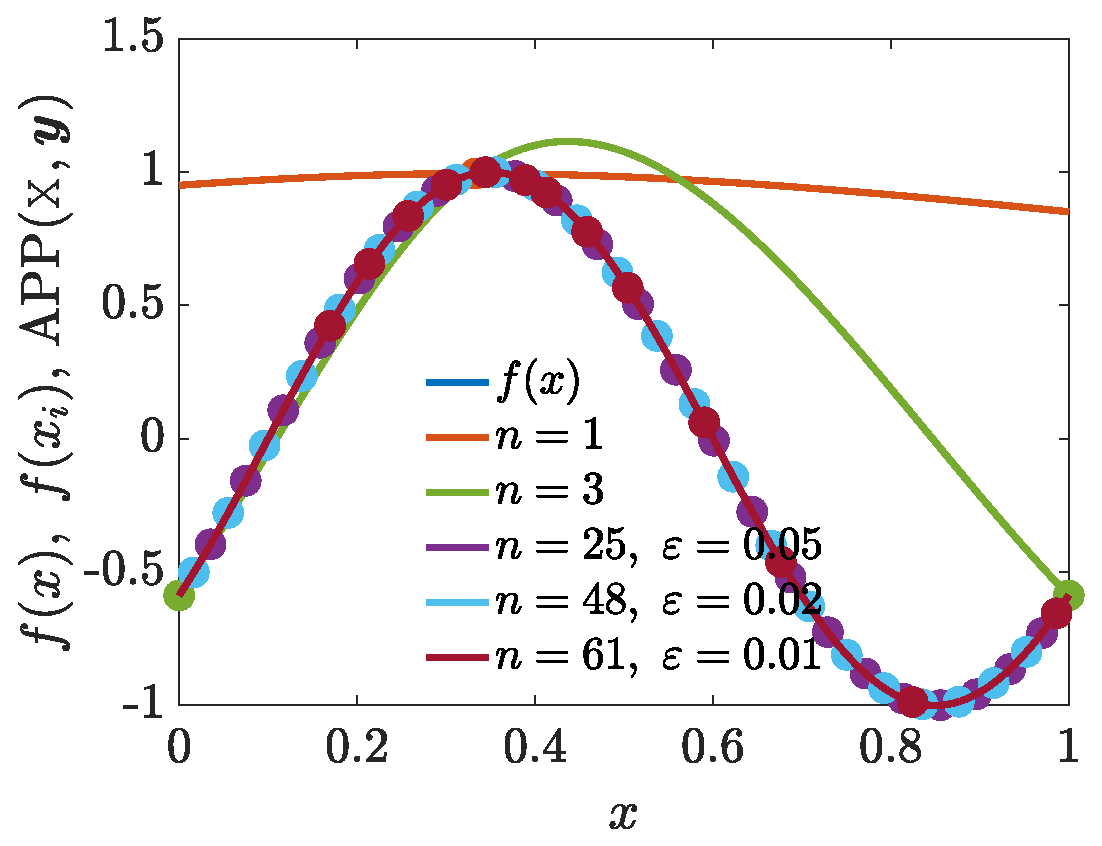
\includegraphics[height = 5.5cm]{ProgramsImages/Alg2_CurrinSineFun_Matern.eps}
		\caption{ \label{fig:ex2}}
	\end{figure}
	
\end{example}

However, unlike Example  \ref{ex:adpsamplesize}, the  pointwise error bounds do not hold for small values of $n$.



Unfortunately, the acquisition function defined in \eqref{eq:nextsample} does not yet depend on the function data, $\by$, but only on the data sites, $\mX$.  In that sense, this algorithm chooses data sites to fill gaps between data sites.  It does not choose data sites more densely where the function  fluctuates more.  In the next section we improve our algorithm to make the acquisition function strongly dependent on $\by$.





%%%%%%%%%%%%%%%%%%%%%%%%%%%%%%%%%%%%%%%%%%%%%%%%%%%%%%%%%%%%%%%%%%%%%%%%%%
%%%%%%%%%%%%%%%%%%%%%%%%%%%%%%%%%%%%%%%%%%%%%%%%%%%%%%%%%%%%%%%%%%%%%%%%%%
\section{Function Approximation when the Hilbert Space Is Inferred} \label{sec:adaptF}
%%%%%%%%%%%%%%%%%%%%%%%%%%%%%%%%%%%%%%%%%%%%%%%%%%%%%%%%%%%%%%%%%%%%%%%%%%
%%%%%%%%%%%%%%%%%%%%%%%%%%%%%%%%%%%%%%%%%%%%%%%%%%%%%%%%%%%%%%%%%%%%%%%%%%



%%%%%%%%%%%%%%%%%%%%%%%%%%%%%%%%%%%%%%%%%%%%%%%%%%%%%%%%%%%%%%%%%%%%%%
%%%%%%%%%%%%%%%%%%%%%%%%%%%%%%%%%%%%%%%%%%%%%%%%%%%%%%%%%%%%%%%%%%%%%%
\subsection{Inferring the Parameters Defining the Reproducing Kernel} \label{sec:adaptTheta}
%%%%%%%%%%%%%%%%%%%%%%%%%%%%%%%%%%%%%%%%%%%%%%%%%%%%%%%%%%%%%%%%%%%%%%
%%%%%%%%%%%%%%%%%%%%%%%%%%%%%%%%%%%%%%%%%%%%%%%%%%%%%%%%%%%%%%%%%%%%%%

So far, we have assumed that the function to be approximation belongs to a fixed RKHS.  However, unless there is strong a priori knowledge, there is no way to know whether our $f$ is typical for  the RKHS chosen.  We do not expect a unique RKHS for which $f$ is typical, but we want to infer a \emph{suitable} RKHS from the data.  

Let $\{\calf_{\btheta} : \btheta \in \Theta\}$ be a family of RKHSs parameterized by $\btheta$.  An example is a generalization of the Mat\'ern kernel  in \eqref{eq:MaternOne}:
\begin{equation} \label{eq:MaternTheta}
K_\btheta(\bt,\bx) = (1 +  \norm{\btheta \odot (\bt-\bx)}) \exp(-\norm{\btheta \odot (\bt-\bx)}),
\end{equation}
where $\odot$ denotes the Hadamard or term-by-term product.  From this section forward, we highlight the dependence of the reproducing kernel and related quantities on $\btheta$.

Figure \ref{fig:MaternThPlot} displays the Mat\'ern reproducing kernel for $d=1$ for three different values of $\btheta = \theta$.  Under this parameterization, the kernel becomes flatter for small $\theta$ and more peaked for large $\theta$.  

\begin{figure}[H]
	\centering
	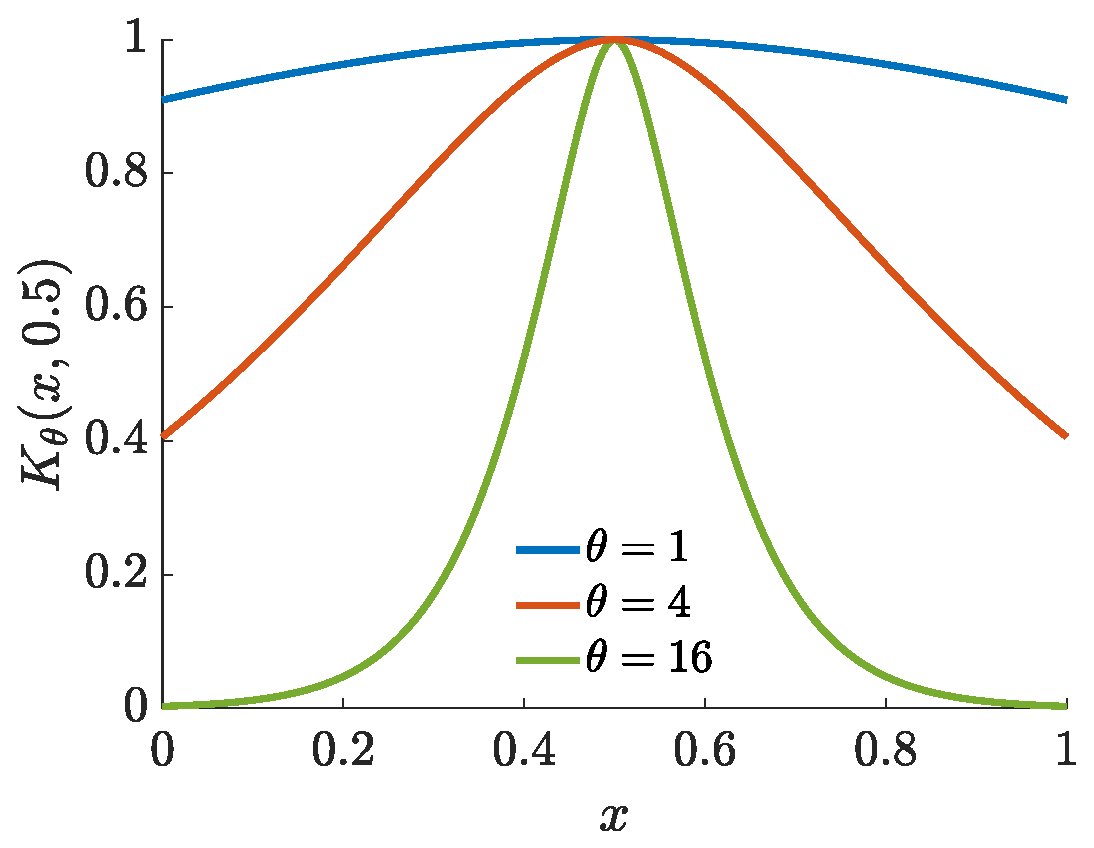
\includegraphics[height = 5.5cm]{ProgramsImages/KthetaPlot.eps} \qquad
	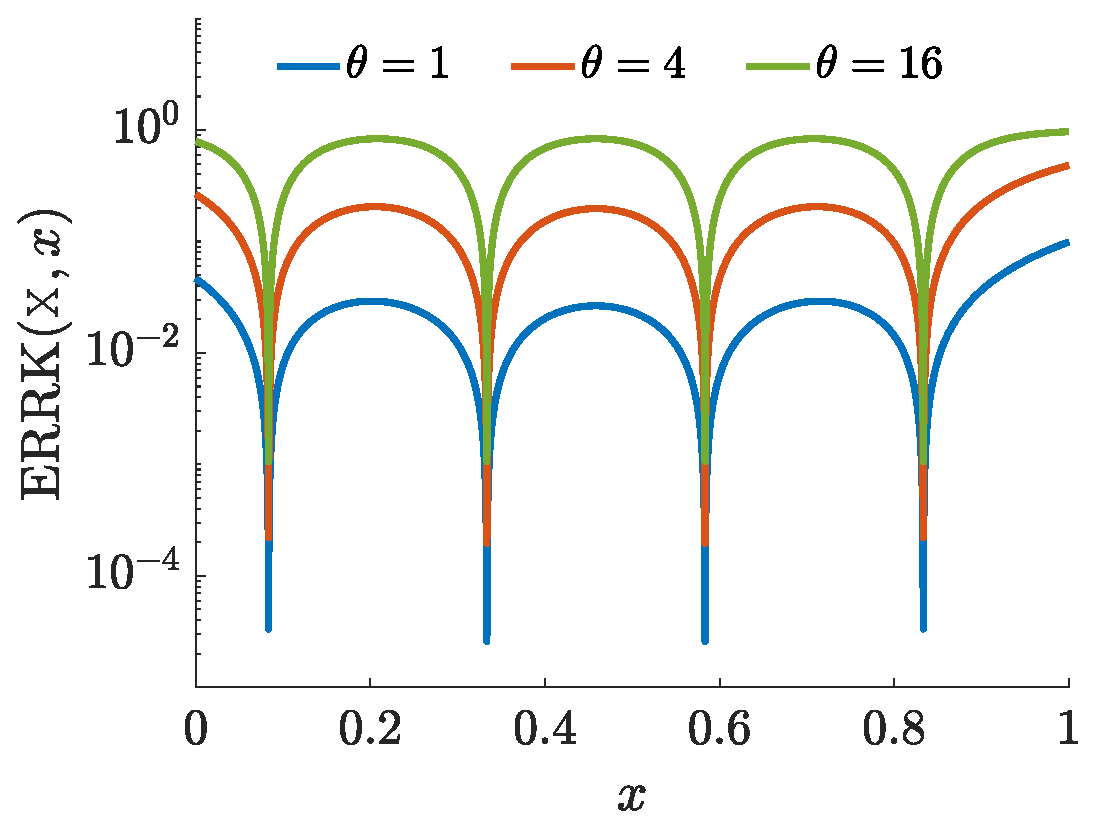
\includegraphics[height = 5.5cm]{ProgramsImages/errKplotth.eps}
	\caption{The Mat\'ern kernel defined in \eqref{eq:MaternTheta} for various values of $\btheta$ \label{fig:MaternThPlot}}
\end{figure}

These differences in kernel shape translate into assumptions about the functions in the RKHS.  Every reproducing kernel describes how large function values may be and how far apart two function values at different locations may be:
\begin{equation} \label{eq:diff_f}
\sup_{\norm[\calf_{\btheta}]{f} \le 1} \abs{f(\bx)}^2 = K_\btheta(\bx,\bx), \qquad    \sup_{\norm[\calf_{\btheta}]{f} \le 1} \abs{f(\bt) - f(\bx)}^2 = K_{\btheta}(\bt,\bt) +  K_{\btheta}(\bx\bx) - 2 K_{\btheta}(\bt,\bx).
\end{equation}
These upper bounds are with respect to the $\calf_\btheta$-norm of the function.  For the Mat\'ern kernel in \eqref{eq:MaternTheta} these statements correspond to 
\begin{equation} \label{eq:diff_f_Matern}
\sup_{\norm[\calf_{\btheta}]{f} \le 1} \abs{f(\bx)}^2 = 1, \qquad 
\sup_{\norm[\calf_{\btheta}]{f} \le 1} \abs{f(\bt) - f(\bx)}^2 = 2[1 - (1 +  \norm{\btheta \odot (\bt-\bx)}) \exp(-\norm{\btheta \odot (\bt-\bx)})].
\end{equation}
For small $\theta$ function values in the RKHS characterized by the Mat\'ern kernel do not vary much with location. For large $\theta$ function values in the RKHS may vary quite a bit over short distances.

These variations in kernel shape affect our function approximation and error bound. quantities in our function approximation algorithm.


The value of $\btheta$ strongly affects the values of $\errK(\mX)$, $A(\mX)$, and 

\FredNote{Perhaps show some figures of how $\errK(\mX,\bx)$ and $A(\mX)$ vary with $\btheta$ and the importance of choosing the correct $\btheta$}

Let $\vBall$ denote the volume of a unit ball in $n$ dimensions, and let $\vEll(\btheta,\mX,\by)$ denote the volume of the ellipsoidal solid in $\reals^n$ consisting of all possible function data whose minimum-norm interpolants have an $\calf_{\btheta}$-norm no greater than that of the observed interpolant:
\begin{align*}
\vEll(\btheta,\mX,\by) &= \vol\bigl(\{ \bz \in \reals^n : \norm[\calf_{\btheta}]{\APP_{\btheta}(\mX,\bz)}  \le \norm[\calf_{\btheta}]{\APP_{\btheta}(\mX,\by)} \} \bigr) \\
& = \vol\Bigl( \bigl \{ \bz \in \reals^n : \bz^T \mK_\btheta^{-1} \bz \le \by^T \mK_\btheta^{-1} \by  \bigr \} \Bigr) \\
& = \vBall \sqrt{\det(\mK_{\btheta})  \, [\by^T \mK_\btheta^{-1} \by]^n } \qquad \text{by \cite{bibid}}
\end{align*}

The volume of the ellipsoidal solid, $\vEll(\btheta,\mX,\by)$, is a measure of how large the observed function data is with respect to the Hilbert space $\calf_{\btheta}$.  This measure is independent of the vertical scale of the reproducing kernel.  It does not change if the reproducing kernel $K_\btheta$ is replaced by $cK_{\btheta}$ for any positive constant $c$.  

Figure \ref{fig:ellipPlot} displays the one-dimensional Mat\'ern kernel in \eqref{eq:MaternTheta} for three different values of $\btheta = \theta$ and the corresponding  ellipsoidal solids $\{ \bz \in \reals^n : \bz^T \mK_\btheta^{-1} \bz \le \by^T \mK_\btheta^{-1} \by  \bigr \}$  defined for a two-sample design.  Here, the ellipsoid corresponding to $\theta = 2$ has the smallest volume (area).


\begin{figure}[H]
	\centering
	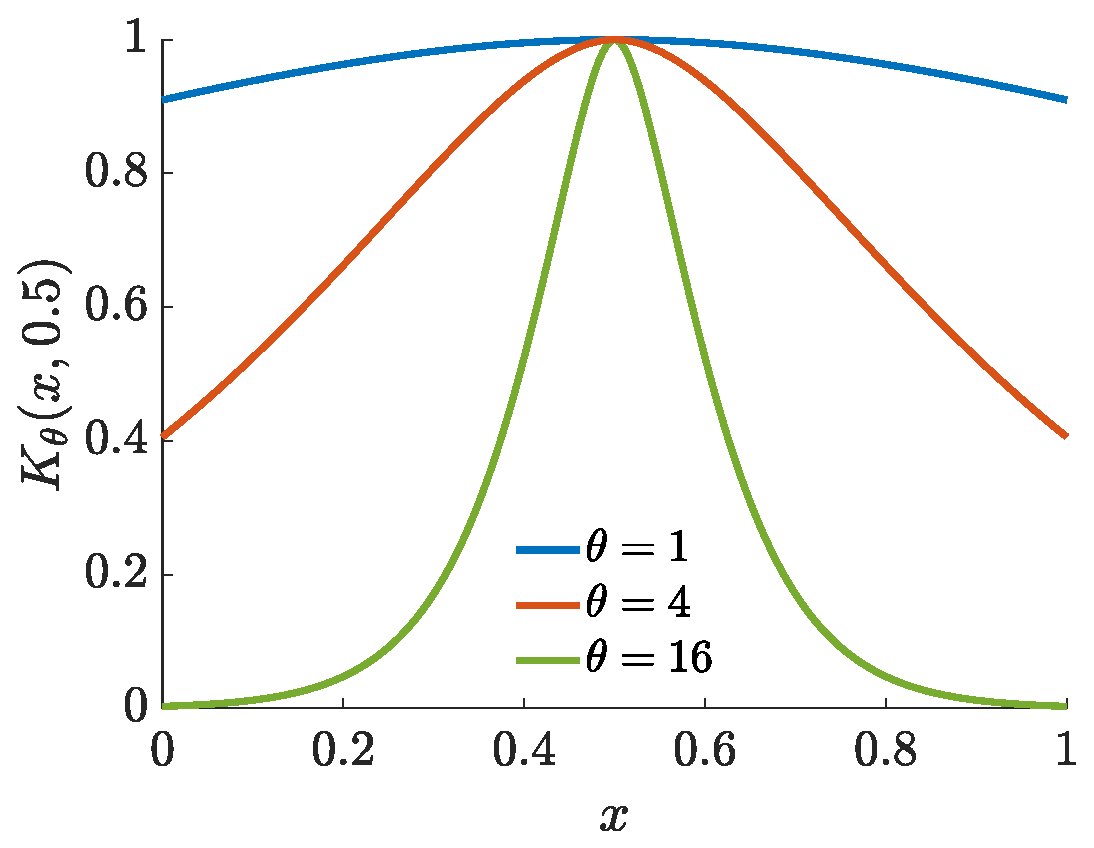
\includegraphics[height = 6cm]{ProgramsImages/KthetaPlot.eps} \qquad
	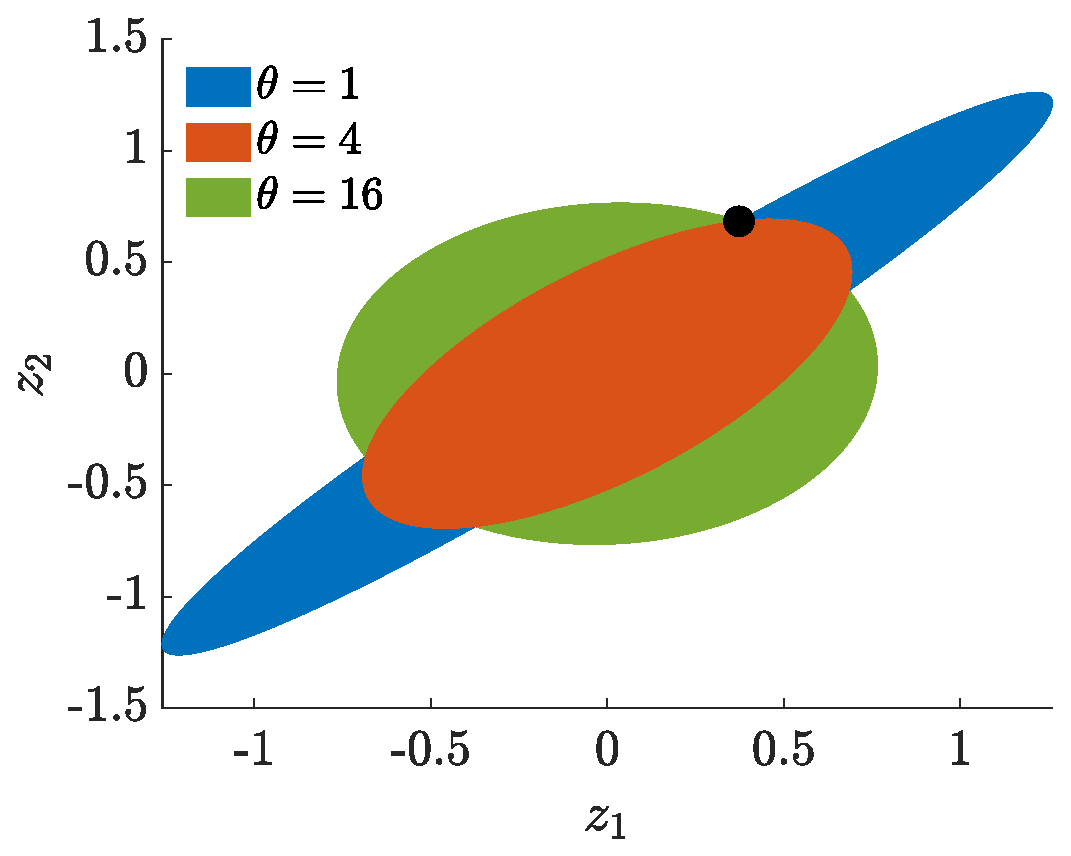
\includegraphics[height = 6cm]{ProgramsImages/ellipsesPlot.eps}
	\caption{The ellipsoidal solids $\{ \bz \in \reals^n : \bz^T \mK_\btheta^{-1} \bz \le \by^T \mK_\btheta^{-1} \by  \bigr \}$ for the Mat\'ern kernel defined in \eqref{eq:MaternTheta}, various values of $\btheta$, and $\by = f(\mX)$, where $\mX = (0.3, 0.6)^T$ and $f$ is defined in ?? \label{fig:ellipPlot}}
\end{figure}

The reproducing kernel describes how large function values may be and how far apart two values of a function at different locations may be:
\begin{equation} \label{eq:diff_f}
\sup_{\norm[\calf_{\btheta}]{f} \le 1} \abs{f(\bx)}^2 = K_\btheta(\bx,\bx), \qquad    \sup_{\norm[\calf_{\btheta}]{f} \le 1} \abs{f(\bt) - f(\bx)}^2 = K_{\btheta}(\bt,\bt) K_{\btheta}(\bx\bx) - 2 [K_{\btheta}(\bt,\bx)]^2.
\end{equation}
For the Mat\'ern kernel in \eqref{eq:MaternTheta} this corresponds to 
\begin{equation} \label{eq:diff_f_Matern}
\sup_{\norm[\calf_{\btheta}]{f} \le 1} \abs{f(\bx)}^2 = 1, \qquad 
\sup_{\norm[\calf_{\btheta}]{f} \le 1} \abs{f(\bt) - f(\bx)}^2 = 1 - 2 [(1 +  \norm{\btheta \odot (\bt-\bx)}) \exp(-\norm{\btheta \odot (\bt-\bx)})]^2.
\end{equation}
The Mat\'ern kernel with small $\theta$ is relatively flat, which means that function values in this RKHS do not vary much with location.  This explains why the ellipsoidal solid for $\theta = 0.5$ hugs the line $z_1 = z_2$.  For large $\theta$ the Mat\'ern kernel is peaked, which explains why the ellipsoidal solid for $\theta = 8$ is more spherical in shape.

We argue that the most suitable kernel is the one that minimizes the volume of the ellipsoidal solid, i.e., the RKHS for which the observed function data is small.   Our choice of $\btheta$ is
\begin{equation} \label{eq:thetEB}
\btheta  =  \argmin_{\theta'}  \vEll(\btheta' ,\mX,\by) 
 = \argmin_{\theta'}  \left[\frac 1n \log \bigl( \det(\mK_{\btheta'}) \bigr) + \log \bigl ( \by^T \mK_{\btheta'}^{-1} \by \bigr)\right].
\end{equation}

Inferring the reproducing kernel from the data necessitates a new candidate cone of functions to be approximated:
\begin{multline} \label{eq:RKHSconeTheta}
\calc : = \biggl \{f \in \bigcup_{\btheta' \in \Theta} \calf_{\btheta'} : \bignorm[\calf]{f - \APP_{\btheta}(f)} \le A_{\btheta}(\mX) \bignorm[\calf]{\APP_{\btheta}(\mX,\by)} \quad \forall \mX \in \Omega^d, \ \by = f(\mX),  \\
 \btheta = \argmin_{\theta'}  \left[\frac 1n \log \bigl( \det(\mK_{\btheta'}) \bigr) + \log \bigl ( \by^T \mK_{\btheta'}^{-1} \by \bigr)\right] \biggr \}.
\end{multline}
This candidate cone is neither a subset or superset of the candidate cone defined in \eqref{eq:RKHScone}.  Since it includes elements of multiple RKHSs, this new candidate cone is not a subset of the earlier one.  On the other hand, the condition that  the norm of the approximation error  is bounded by the norm of the approximation for \emph{whatever} $\btheta$ our criterion selects is a stricter condition than what is required in \eqref{eq:RKHScone}. 


\begin{algorithm}[H]
	\caption{Adaptive Data Site and RKHS Selection and Adaptive Sample Size \label{alg:adapttheta}}
	\begin{algorithmic}
		\PARAM the family of RKHSs, $\{\calf_{\btheta} : \btheta \in \Theta\}$; $A_\infty$ and $B_0$, which define the candidate cone, $\cc$, in \eqref{eq:RKHSconeTheta}; an initial data site, $\bx_1$
		\INPUT a black-box function, $f \in \cc$; an absolute error tolerance, $\varepsilon>0$
		
		\Ensure Error criterion $\norm[\infty]{f - \ALG(f,\varepsilon)} \le \varepsilon$
		
		\State Let $n \leftarrow 0$
		
		\Repeat
		
		\If{ $n > 0$}
		
		\State Let $ \bx_{n+1} = \displaystyle \argmax_{\bx \in \Omega} \errK(\mX,\bx)$
		
		\EndIf
		
		\State Let $n \leftarrow n + 1$
		
		\State Update $\displaystyle\btheta = \argmin_{\theta'}  \left[\frac 1n \log \bigl( \det(\mK_{\btheta'}) \bigr) + \log \bigl ( \by^T \mK_{\btheta'}^{-1} \by \bigr)\right]$
		
		\State Compute $\by$, $A_\btheta(\mX)$, $\mK_\btheta = K_\btheta(\mX,\mX)$, and $K_\btheta(\mX,\cdot)$
		
		\Until  $A(\mX) \errK(\mX) \sqrt{ \by^T \mK^{-1} \by }  \le \varepsilon$
		
		\RETURN $\ALG(f,\varepsilon) = \by^T \mK^{-1} K(\mX,\cdot)$
		
	\end{algorithmic}
\end{algorithm}

Because $\btheta$ must be chosen by optimization, the asymptotic computational cost of Algorithm \ref{alg:adapttheta} is more than the earlier two algorithms.  Let $\Ntheta$ denote the number of $\btheta'$ values that must be tried at each step in the algorithm to obtain the optimum, $\btheta$.  The objective function for this optimization requires $\Order(n^3)$ operations to evaluate.  Moreover, since $\btheta$ may change for each $n$, the data-based error bound in the stopping criterion requires an evaluation of the sup-norm from scratch.  Therefore, the total cost of the algorithm is 
\begin{equation} \label{eq:compcosttheta}
\Order\bigl(\$(f)n + \Ntheta n^4 + \NT n^3 \bigr),
\end{equation}
where $n$ is the final number of data sites required.  Again, our intended application is that for which $\$(f)$ dominates $\Ntheta n^3$ and $\NT n^2$.  

\FredNote{Example again. Show how inferring $\btheta$ helps.}

\begin{example}
	\label{ex:adpdatachooseth}
	Consider again the function to be approximated as in Examples \ref{ex:adpsamplesize} and \ref{ex:adpdataselect}, but now with the Mat'ern kernel \eqref{eq:MaternTheta} where the parameter $\btheta = \theta$ is inferred from the data as in Algorithm \ref{alg:adapttheta}.
		
	\input{ProgramsImages/Alg3_OutCurrinSineFun_Matern.txt}
	
	
	\begin{figure}[H]
		\centering
		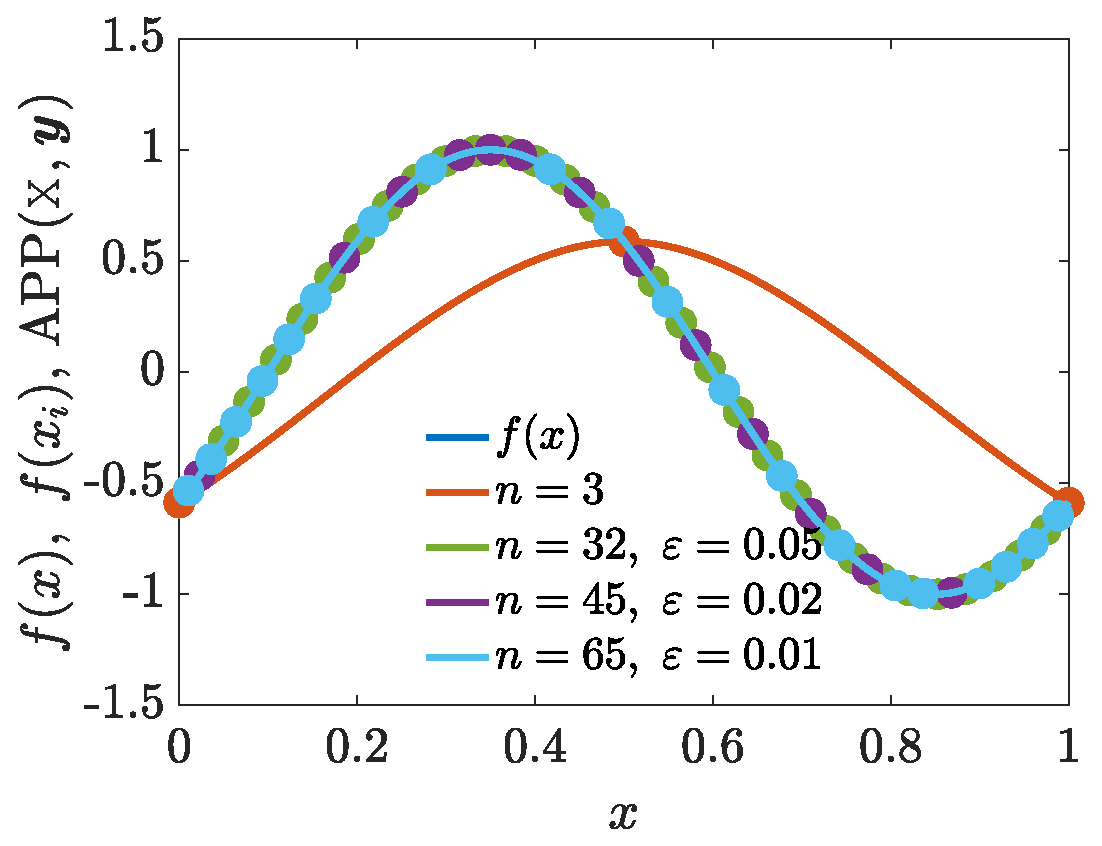
\includegraphics[height = 5.5cm]{ProgramsImages/Alg3_CurrinSineFun_Matern.eps}
		\caption{ \label{fig:ex3}}
	\end{figure}
	
\end{example}




%%%%%%%%%%%%%%%%%%%%%%%%%%%%%%%%%%%%%%%%%%%%%%%%%%%%%%%%%%%%%%%%%%%%%%
%%%%%%%%%%%%%%%%%%%%%%%%%%%%%%%%%%%%%%%%%%%%%%%%%%%%%%%%%%%%%%%%%%%%%%
\subsection{A Bayesian Numerical Analysis Digression} \label{sec:Bayes}
%%%%%%%%%%%%%%%%%%%%%%%%%%%%%%%%%%%%%%%%%%%%%%%%%%%%%%%%%%%%%%%%%%%%%%
%%%%%%%%%%%%%%%%%%%%%%%%%%%%%%%%%%%%%%%%%%%%%%%%%%%%%%%%%%%%%%%%%%%%%%

Bayesian numerical analysis \cite{Dia88a,RasWil06a,Ste99} provides a parallel approach to the deterministic analysis presented here.  Bayesian function approximation assumes that the function to be approximated is a stochastic process, often a Gaussian process with zero mean and covariance kernel $s^2 K_\btheta(\cdot, \cdot)$.  This means that 
\begin{equation*}
\Ex[f(\bx)] = 0, \quad \Ex[f(\bt) f(\bx)] = s^2K_\btheta(\bt,\bx), \qquad \forall \bt, \bx \in \cx.
\end{equation*}
The posterior mean value of $f(\bx)$ given the data $f(\bx) = \by$, takes the same form as $\APP_\btheta(\mX,\by)(\bx)$ in \eqref{eq:RKHSAPP}.  Moreover, the posterior standard deviation of $f(\bx)$, using empirical Bayes to estimate the parameters $s$ and $\btheta$ is \cite{Hic17a,??}
\begin{equation*}
\sqrt{\frac 1n \norm[\infty]{K_\btheta(\cdot,\cdot) - K_\btheta(\cdot,\mX) \mK_\btheta^{-1} K_\btheta(\mX,\cdot)} \, [\by^T \mK_\btheta^{-1} \by] }, \qquad \btheta = \argmin_{\theta'}  \left[\frac 1n \log \bigl( \det(\mK_{\btheta'}) \bigr) + \log \bigl ( \by^T \mK_{\btheta'}^{-1} \by \bigr)\right].
\end{equation*}

The selection criterion proposed above in \eqref{eq:thetEB} is inspired by the empirical Bayes criterion here, however, our justification is geometric and does not require a Bayesian setting.  The pointwise data-based error bound in \eqref{eq:DataErrBdA} above is similar to the posterior standard deviation of $f(\bx)$ here, but with the design dependent factor $A(\mX)$ instead of $1/\sqrt{n}$.


%%%%%%%%%%%%%%%%%%%%%%%%%%%%%%%%%%%%%%%%%%%%%%%%%%%%%%%%%%%%%%%%%%%%%%
%%%%%%%%%%%%%%%%%%%%%%%%%%%%%%%%%%%%%%%%%%%%%%%%%%%%%%%%%%%%%%%%%%%%%%
\subsection{Inferring the Location Dependence of the Reproducing Kernel} \label{sec:InferSpace}
%%%%%%%%%%%%%%%%%%%%%%%%%%%%%%%%%%%%%%%%%%%%%%%%%%%%%%%%%%%%%%%%%%%%%%
%%%%%%%%%%%%%%%%%%%%%%%%%%%%%%%%%%%%%%%%%%%%%%%%%%%%%%%%%%%%%%%%%%%%%%

Although the function data, $\by$, appears in the selection criterion for $\btheta$, the form of reproducing kernel that we have considered thus far does not allow us to deduce that the function may vary more in one part of the domain than another.  The adaptive design defined by \eqref{eq:nextsample} may still be a space-filling design only slightly influenced by the observed function data.

\FredNote{Insert Example}
\begin{example}
\label{ex:compfun}
To illustrate it is still a space-filling design,  we consider the following univariate function, which has a mean value near zero
	\begin{equation}
	f: x \mapsto 
 \exp(-6x)\sin(8x+0.1) - 0.1,  \qquad x \in [0,1],
	\end{equation}
	which is plotted in Figure \ref{fig:ex4a}. 
		
	\begin{figure}[H]
		\centering
		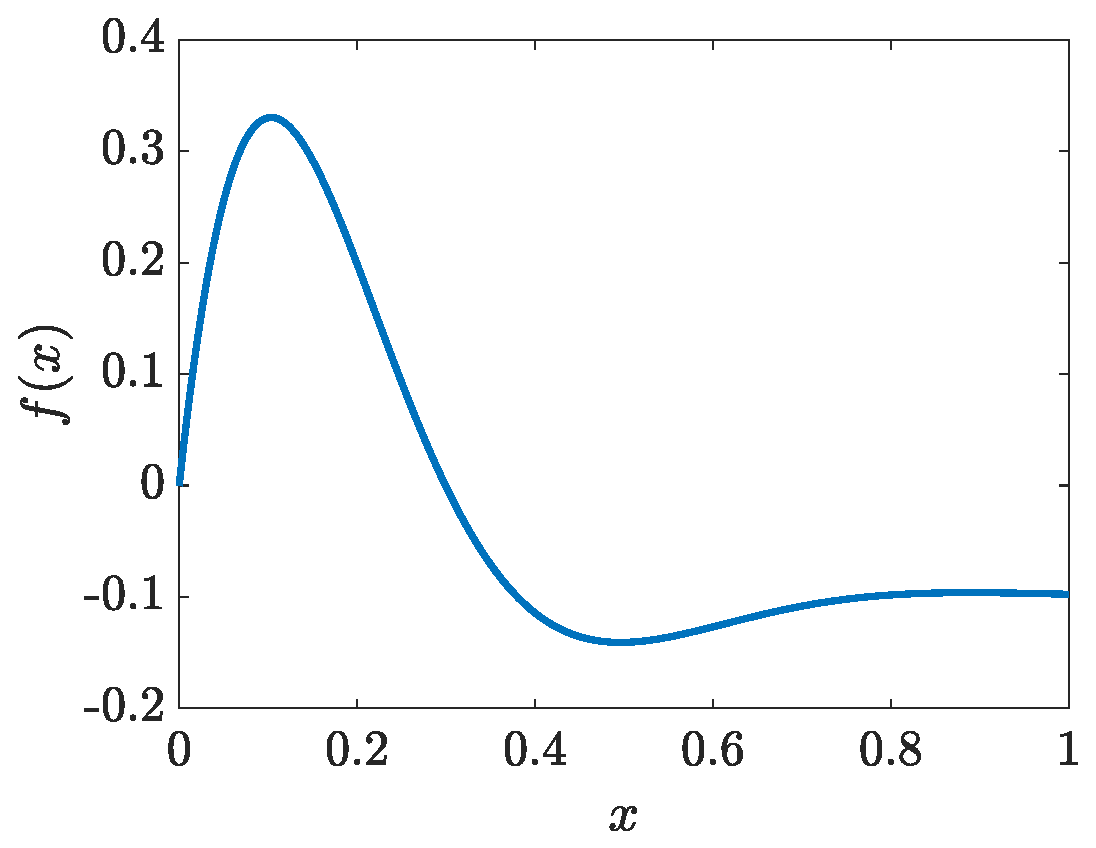
\includegraphics[height = 4.5cm]{ProgramsImages/LeftPeakFunPlot.eps} \qquad
		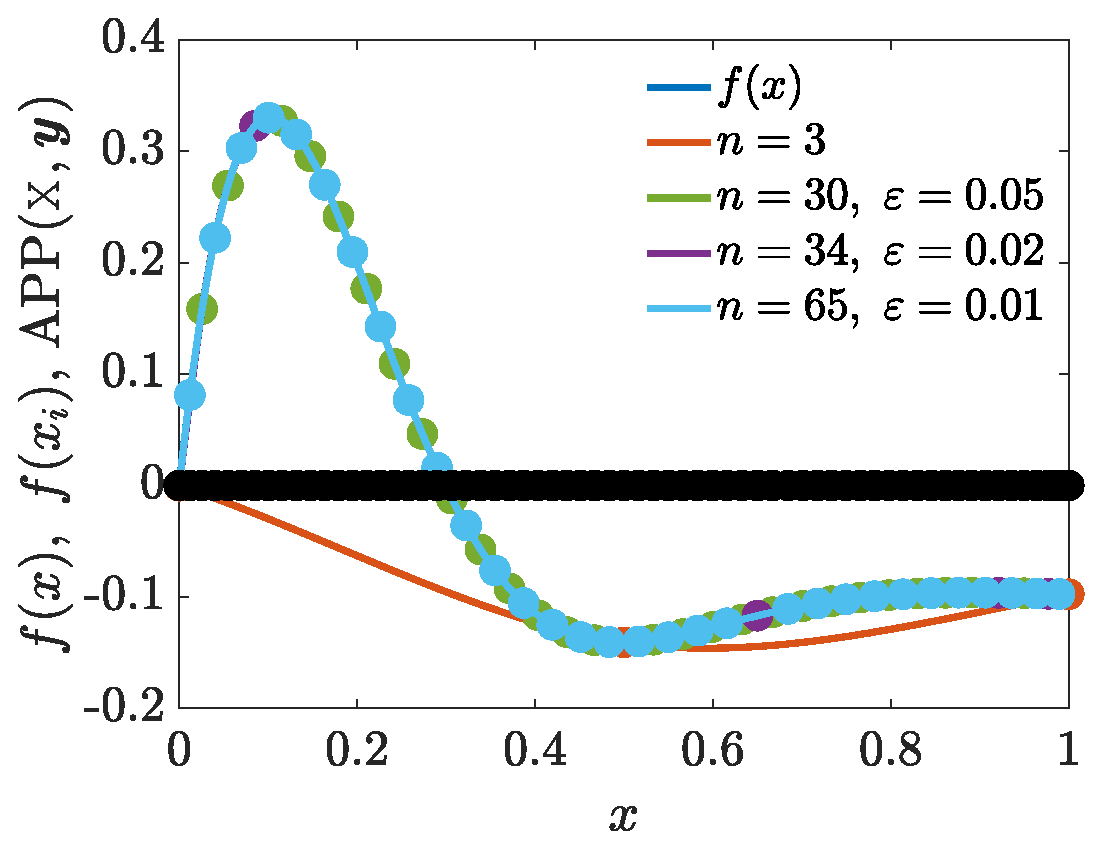
\includegraphics[height = 4.5cm]{ProgramsImages/Alg3_LeftPeakFun_Matern.eps} \qquad		
		\caption{ \label{fig:ex4a}}
	\end{figure}
	We apply Algorithm \ref{alg:adapttheta} to this example using the sequence of data sites described in \eqref{eq:FixedVDCDes} with $n_0=3$. We choose the generalization of the Mat\'ern kernel in \eqref{eq:MaternOne},  $A_\infty =1, B_0 = 0.05$, and $\mT = (0, 0.001, \ldots, 1)^T$. 
	


		
	\input{ProgramsImages/Alg3_OutLeftPeakFun_Matern.txt}

\end{example}

 
In the example above the function oscillates more on the left than the right, but \eqref{eq:diff_f_Matern} for the Mat\'ern kernel says that the maximum difference between function values at two locations is only depends on the distance between the locations.  The same holds for all $K(\bt ,\bx)$ that are  functions of $\bt - \bx$.  Even for more general kernels, we want to be able to infer their location dependence from the data, not have it baked in.

For any reproducing kernel, $K(\bt ,\bx)$, it follows that $w(\bt)w(\bx)K(\bt ,\bx)$ is also a reproducing kernel regardless of the choice of $w$.  We can generalize the Mat\'ern kernel in \eqref{eq:MaternTheta} further as follows and apply \eqref{eq:diff_f}:
\begin{align} \label{eq:MaternAB}
K_\btheta(\bt,\bx) &= \exp(\bb^T(\bt + \bx))(1 +  \norm{\ba \odot (\bt-\bx)}) \exp(-\norm{\ba \odot (\bt-\bx)}),  \quad \btheta=(\ba, \bb), \\
\nonumber
%\label{eq:diff_f_MaternAB}
\sup_{\norm[\calf_{\btheta}]{f} \le 1} \abs{f(\bx)}^2 &= \exp(2\bb^T\bx), \\
\nonumber
\MoveEqLeft[4]{\sup_{\norm[\calf_{\btheta}]{f} \le 1} \abs{f(\bt) - f(\bx)}^2} = \\
\nonumber 
& \qquad \exp(2\bb^T(\bt + \bx))\{ 1 - 2 (1 +  \norm{\ba \odot (\bt-\bx)}) \exp(-\norm{\ba \odot (\bt-\bx)})]^2\}.
\end{align}
Now, the size of the function values and the difference between function values at different locations can rise or fall depending on the parameter $\bb$, which can be inferred from the data.


\FredNote{Repeat Example with new kernel}

Now the kernel is strongly dependent on $\by$

\begin{example}
\label{ex:compfun2}
	\begin{figure}[H]
		\centering
		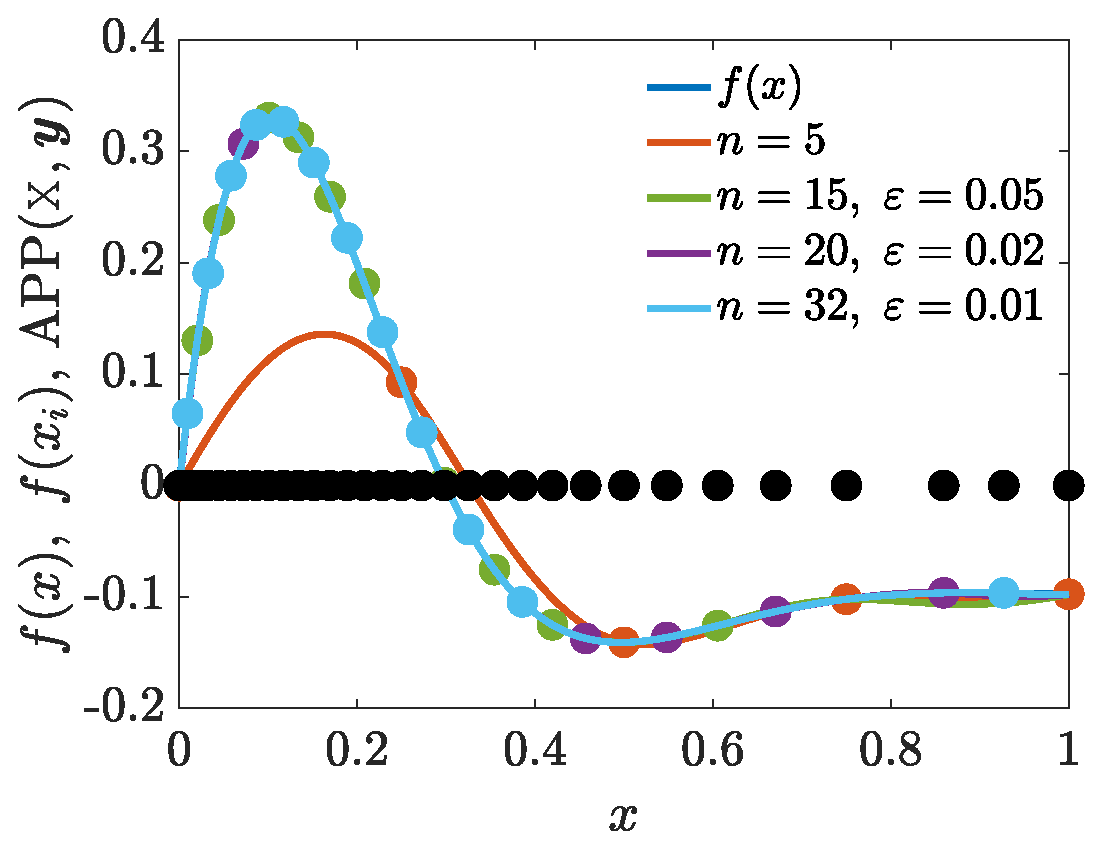
\includegraphics[height = 5.5cm]{ProgramsImages/Alg3_LeftPeakFun_SpatialMatern.eps} 
		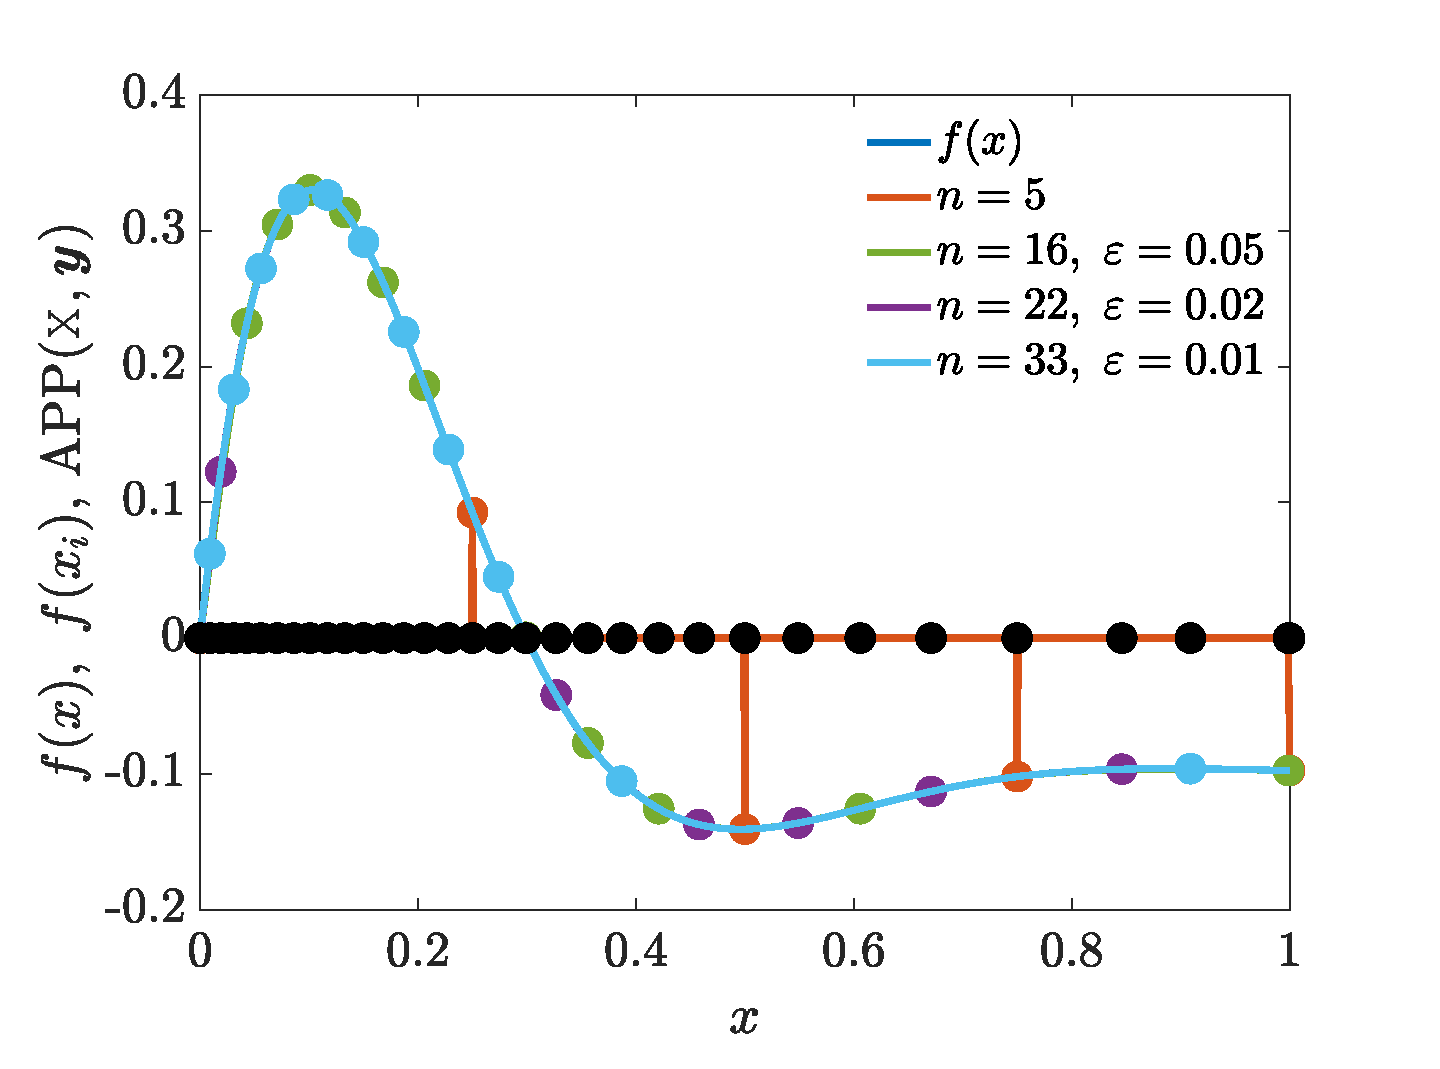
\includegraphics[height = 5.5cm]{ProgramsImages/Alg3_LeftPeakFun_SpatialMatern2.eps} 
		\caption{ \label{fig:ex5}}
	\end{figure}

		
	\input{ProgramsImages/Alg3_OutLeftPeakFun_SpatialMatern.txt}


\end{example}

%%%%%%%%%%%%%%%%%%%%%%%%%%%%%%%%%%%%%%%%%%%%%%%%%%%%%%%%%%%%%%%%%%%%%%
%%%%%%%%%%%%%%%%%%%%%%%%%%%%%%%%%%%%%%%%%%%%%%%%%%%%%%%%%%%%%%%%%%%%%%
\section{Recovering Pure Trends Exactly} \label{sec:poly}
%%%%%%%%%%%%%%%%%%%%%%%%%%%%%%%%%%%%%%%%%%%%%%%%%%%%%%%%%%%%%%%%%%%%%%
%%%%%%%%%%%%%%%%%%%%%%%%%%%%%%%%%%%%%%%%%%%%%%%%%%%%%%%%%%%%%%%%%%%%%%

The algorithm developed so far must be extended to recover even constant functions exactly.  Let $\calf_t$ be a finite dimensional vector space of possible \emph{trends} with basis $\{p_1, \ldots, p_s\}$.  For example, it might be space of polynomials.  We think of $\calf_{\btheta}$ as the infinite dimensional space of possible \emph{fluctuations} around the trend.  So, our function to be approximated, $f$, lies in the vector space $\calh_\btheta := \calf_t \oplus \calf_\btheta$ with the following semi-norm that measures the size of its fluctuation:
\begin{equation} \label{eq:seminorm} 
\abs{f}_{\calh_\btheta} = \min \{ \norm[\calf_\btheta] {f_\btheta} : f = f_t + f_\btheta, \ f_t \in \calf_t, \ f_\btheta \in \calf_\btheta \}.
\end{equation}
It is possible to have a non-unique decomposition of $f$ into a trend and fluctuation.

We modify our approximation in \eqref{eq:RKHSAPP} to include a trend
\begin{subequations} \label{eq:RKHSAPP_P}
	\begin{align} 
	\APP_\btheta(\mX,\by) &= \sum_{i=1}^n c_i K_\btheta(\bx_i,\cdot) + \sum_{j=1}^s \gamma_i p_j = \bc^T K_\btheta(\mX,\cdot) + \bgamma^T \bp(\cdot) \in \calf_{\btheta \mX}, \\
	\label{eq:RKHSAPP_PB}
	\text{where } & \qquad \begin{pmatrix} \bc \\ \bgamma \end{pmatrix} = 
	\begin{pmatrix} \mK_\btheta  & \mP \\ \mP^T & \mZero_s \end{pmatrix}^{-1} 
	\begin{pmatrix}\by \\ \bzero_s \end{pmatrix}, 
	\quad \mK_\btheta = K_\btheta(\mX,\mX) = \bigl( K_\btheta(\bx_i,\bx_j) \bigr)_{i,j=1}^n,  \\
	& \qquad  K_\btheta(\mX,\bx) = \bigl(K_\btheta\bx,\bx_i) \bigr)_{i=1}^n =  K_\btheta(\bx, \mX)^T, \quad \mP = \bp^T(\mX) = \bigl( p_j(\bx_i)\bigr )_{i,j=1}^{n,s}.
	\end{align}
\end{subequations}
We assume that $\mP$ has full rank and that $\mK$ is invertible. Then the solution of \eqref{eq:RKHSAPP_PB} is
\begin{equation}
\bc = \mM_\btheta \by, \quad \mM_\btheta := \mK_\btheta^{-1} - \mK_\btheta^{-1}\mP (\mP^T \mK_\btheta^{-1} \mP)^{-1} \mP^T \mK_\btheta^{-1}, \qquad
\bgamma = (\mP^T \mK_\btheta^{-1} \mP)^{-1} \mP^T \mK_\btheta^{-1} \by.
\end{equation}
Note that if $f$ is pure trend, i.e., $f = \balpha^T \bp \in \calf_t$ for some constant $\balpha$, then $\APP_\btheta(\mX,\by) = \balpha^T \bp$ by straightforward calculation.  So our approximation recovers pure trends exactly.


For any design $\mX$ and function data $\by$, let $\calg_\btheta(\mX,\by)$ denote the subset of $\calh_\btheta$ that interpolates the data, i.e., $\calg_\btheta(\mX,\by) := \{ g = g_t + g_{\btheta} : g_t \in \calf_t, \ g_{\btheta} \in \calf_{\btheta}, \ g(\mX)  = \by\}$.  
Then, $\APP_\btheta(\mX,\by)$ is the minimum semi-norm interpolant, i.e., $\APP_\btheta(\mX,\by) = \argmin_{g \in \calg(\mX,\by)}  \abs{g}_{\calh_\btheta}$.  This property of  $\APP_\btheta(\mX,\by)$ is related to the fact that  $\APP_\btheta(\mX,\by)$ exactly reproduces all trends.

The function, $f$, to be approximated is the sum of three parts: $f_t = (\bgamma + \bdelta)^T \bp \in \calf_t$,  $f_{\btheta \mX} = (\bc + \bDelta)^T K_\btheta(\mX,\cdot) \in \calf_{\btheta \mX}$ and $f_{\btheta \mX \perp} \in \{g \in \calf_\btheta : g(\mX) = \bzero\} \in \calf_{\btheta \mX \perp}$.  The interpolation condition implies that, $\mK_\btheta \bDelta  + \mP \bdelta = \bzero$, so $\bDelta = - \mK_\btheta^{-1} \mP \bdelta$.  The error in approximating $f$ by $\APP_\btheta(\mX,\by)$ is comprised of two parts: i) the error in approximating $f_t + f_{\btheta \mX}$ by $\APP_\btheta(\mX,\by)$, and ii) $f_{\btheta \mX \perp}$.  The latter part is bounded as in \eqref{eq:RKHSErrBd}, but the former part is absent in \eqref{eq:RKHSErrBd}: 
\begin{align}
\label{eq:RKHSErrBdP}
\abs{f(\bx) - \APP(\mX,\by)(\bx)}
& \le \abs{ f_t(\bx) + f_\btheta(\bx) - \APP(\mX,\by)(\bx)} + \abs{f_{\btheta\perp}(\bx)} 
\\
\nonumber
& = \abs{ \bdelta^T [\bp(\bx)- \mP^T \mK_\btheta^{-1}K_\btheta(\mX,\bx)  ] } + \errK(\mX,\bx) \norm[\calf_\btheta]{f_{\btheta\perp}(\bx)}
\\
\nonumber
& \le \errP(\mX,\bx) \norm{\bdelta} + \errK(\mX,\bx) \norm[\calf_\btheta]{f_{\btheta\perp}(\bx)},
\end{align}
where
\begin{equation}
\errP(\mX,\bx)  : = \sqrt{\bp^T(\bx)\bp(\bx) - 2 \bp^T(\bx)\mP^T \mK_\btheta^{-1}K_\btheta(\mX,\bx)  
	+  K_\btheta(\bx,\mX)  \mK_\btheta^{-1} \mP \mP^T \mK_\btheta^{-1}K_\btheta(\mX,\bx)  }
\end{equation}

As was done in Section \ref{sec:basicIdea}, we must assume that $f$ lies in a cone of functions for which $\norm{\delta}$ and $\norm[\calf_\btheta]{f_{\btheta\perp}(\bx)}$ are bounded by quantities derived from data.  This allows us to  construct a data-driven error bound for our approximation to $f$.  We assume that the error in the coefficient of the trend in $f$ is not much larger than the  coefficient of the trend in $\APP(\mX,\by)$, i.e., 
\begin{gather*}
\norm{\bdelta} \le A_{t\btheta}(\mX) \norm{\bgamma}, \qquad A_{t\btheta}(\mX): = \begin{cases} \displaystyle
\frac{A_{t\infty} B_{t0}}{B_{t0} - B_{t \btheta}(\mX)}, & B_{t \btheta}(\mX) < B_{t0}, \\
\infty, & B(\mX) \ge B_{t0}.
\end{cases}\\
B_{t\btheta}(\mX) : =   \frac{\errP(\mX)}{\sqrt{\norm[\infty]{\bp^T(\cdot)\bp(\cdot)}}}, \qquad \errP(\mX) := \norm[\infty]{\errP(\mX,\cdot)}.
\end{gather*} 

We make an analogous assumption as in \eqref{eq:RKHScone} for the norm of $f_{\btheta \perp}$ being bounded in terms of the norm of the part of $\APP(\mX,\by)$ lying in $\calf_{\btheta \mX}$.  Noting that $M_\btheta K_\btheta^{-1} M_\btheta = M_\btheta$.  It follows that $\norm[\calf_{\btheta}]{bc^T K_\btheta(\mX,\cdot)} = \sqrt{\by^T \mM_\btheta \by}$.

As in Section \ref{sec:adaptF}, we assume that $\btheta$ is inferred from data, however, we modify the selection criterion in \eqref{eq:thetEB} by replacing $\mK_\btheta$ by $\mM_{\btheta}^{-1}$.  The geometric interpretation of choosing $\btheta$ to make the data as small as possible still applies, but the ellipsoid solid has a bit different definition.

The candidate cone allowing for trends is now defined as
\begin{multline} \label{eq:RKHSPconeTheta}
\calc : = \biggl \{f \in \calf_t \oplus \bigcup_{\btheta' \in \Theta} \calf_{\btheta'} : 
\bignorm[\calf]{f_{\btheta \perp}} \le A_{\btheta}(\mX) \sqrt{\by^T \mM_\btheta \by} \quad \text{and} \\ 
\norm{\bdelta} \le A_{t \btheta}(\mX) \sqrt{\by^T \mK_\btheta^{-1}\mP (\mP^T \mK_\btheta^{-1} \mP)^{-1} \mP^T \mK_\btheta^{-1} \by} \qquad \forall \mX \in \Omega^d, \ \by = f(\mX),  \\
\text{where }\btheta = \argmin_{\theta'}  \left[\frac 1n \log \bigl( \det(\mM^{-1}_{\btheta'}) \bigr) + \log \bigl ( \by^T \mM_{\btheta'} \by \bigr)\right] \biggr \}.
\end{multline}
A data-driven error bound for functions in this cone follows immediately from \eqref{eq:RKHSErrBdP} and \eqref{eq:RKHSPconeTheta}:
\begin{subequations}  \label{eq:DataErrBdPoly}
\begin{align}
\abs{f(\bx) - \APP(\mX,\by)(\bx)}
& \le A_{t \btheta}(\mX) \errP(\mX,\bx) \sqrt{\by^T \mK_\btheta^{-1}\mP (\mP^T \mK_\btheta^{-1} \mP)^{-1} \mP^T \mK_\btheta^{-1} \by} \\
\nonumber
&\qquad \qquad + A_{\btheta}(\mX) \errK(\mX,\bx) \sqrt{\by^T \mM_\btheta \by} 
=:\ERR(\mX,\by,\bx) \qquad \forall f \in \calc,\\
\norm[\infty]{f - \APP(\mX,\by)}
& \le A_{t \btheta}(\mX) \errP(\mX) \sqrt{\by^T \mK_\btheta^{-1}\mP (\mP^T \mK_\btheta^{-1} \mP)^{-1} \mP^T \mK_\btheta^{-1} \by} \\
\nonumber
&\qquad \qquad + A_{\btheta}(\mX) \errK(\mX)  \sqrt{\by^T \mM_\btheta \by}  
=:\ERR(\mX,\by), \qquad \forall f \in \calc.
\end{align}
\end{subequations}

In contrast to the situation without a trend, the pointwise error bound for the function approximation has two terms, each of which depends on location.  Therefore, our acquisition function used to iteratively choose the next data site should include the whole pointwise error bound.  We choose it to be $\ERR(\mX,\by,\cdot)$.

Our adaptive function algorithm including perfect recovery of pure trends takes the  form below.  It is the culmination of starting with the idea of a candidate cone in Algorithm \ref{alg:basicadapt} and adding additional levels of sophistication.

\begin{algorithm}[H]
	\caption{Adaptive Data Site and RKHS Selection and Adaptive Sample Size; Trends Included \label{alg:trend}}
	\begin{algorithmic}
		\PARAM the family of RKHSs, $\{\calf_{\btheta} : \btheta \in \Theta\}$; $A_\infty$, $B_0$, $A_{t\infty}$, and  $B_{t0}$, which define the candidate cone, $\cc$, in \eqref{eq:RKHSPconeTheta}; an initial data site, $\bx_1$
		\INPUT a black-box function, $f \in \cc$; an absolute error tolerance, $\varepsilon>0$
		
		\Ensure Error criterion $\norm[\infty]{f - \ALG(f,\varepsilon)} \le \varepsilon$
		
		\State Let $n \leftarrow 0$
		
		\Repeat
		
		\If{ $n > 0$}
		
		\State Let $ \bx_{n+1} = \displaystyle \argmax_{\bx \in \Omega} \ERR(\mX,\by,\bx)$
		
		\EndIf
		
		\State Let $n \leftarrow n + 1$
		
		\State Update $\displaystyle\btheta = \argmin_{\theta'}  \left[\frac 1n \log \bigl( \det(\mM^{-1}_{\btheta'}) \bigr) + \log \bigl ( \by^T \mM_{\btheta'} \by \bigr)\right]$
		
		\State Update all necessary quantities to compute the data-driven error bound
		
		\Until  $\ERR(\mX,\by) \le \varepsilon$
		
		\RETURN $\ALG(f,\varepsilon) = \APP(\mX,\by)$ given by \eqref{eq:RKHSAPP_P}
		
	\end{algorithmic}
\end{algorithm}



\FredNote{Summary Theorem}

\begin{theorem}
	The algorithms constructed in this article satisfy absolute error criterion \eqref{eq:errorcrit} under the conditions prescribed below:
	\begin{itemize}
		\item Algorithm \ref{alg:basicadapt} for the candidate cone
		\begin{multline}
		\label{eq:finalconeOne}
		\calc := 
		\Bigl \{f \in \calf : \bignorm[\calf]{f - \APP(f)} \le A(\mX) \bignorm[\calf]{\APP(\mX,\by)} \\
		\bx_1, \bx_2, \ldots \text{ prescribed}, \quad \forall n \ge n_0,  \ \by = f(\mX) \Bigr \},
		\end{multline}
	\end{itemize}
\end{theorem}
%%%%%%%%%%%%%%%%%%%%%%%%%%%%%%%%%%%%%%%%%%%%%%%%%%%%%%%%%%%%%%%%%%%%%%
%%%%%%%%%%%%%%%%%%%%%%%%%%%%%%%%%%%%%%%%%%%%%%%%%%%%%%%%%%%%%%%%%%%%%%
\section{Numerical Experiments}
%%%%%%%%%%%%%%%%%%%%%%%%%%%%%%%%%%%%%%%%%%%%%%%%%%%%%%%%%%%%%%%%%%%%%%
%%%%%%%%%%%%%%%%%%%%%%%%%%%%%%%%%%%%%%%%%%%%%%%%%%%%%%%%%%%%%%%%%%%%%%

\bibliographystyle{amsplain}
\bibliography{FJHown23,FJH23}

%%%%%%%%%%%%%%%%%%%%%%%%%%%%%%%%%%%%%%%%%%%%%%%%%%%%%%%%%%%%%%%%%%%%%%
%%%%%%%%%%%%%%%%%%%%%%%%%%%%%%%%%%%%%%%%%%%%%%%%%%%%%%%%%%%%%%%%%%%%%%
\section*{Appendix}
%%%%%%%%%%%%%%%%%%%%%%%%%%%%%%%%%%%%%%%%%%%%%%%%%%%%%%%%%%%%%%%%%%%%%%
%%%%%%%%%%%%%%%%%%%%%%%%%%%%%%%%%%%%%%%%%%%%%%%%%%%%%%%%%%%%%%%%%%%%%%
The Gram matrix, $\mK$ defined in \eqref{eq:RKHSAPP} is positive definite, and therefore has a Cholesky decomposition, $\mK = \mL \mD \mL^T$, where $\mL$ is a lower unitriangular matrix and $\mD$ is a diagonal matrix with positive diagonal elements.  Moreover, $\mK^{-1} = \mU \mD^{-1} \mU^T$, where $\mU := \mL^{-T}$ is an upper unitriangular matrix. As the sample size grows, these matrices can be constructed recursively.  Expressing the sample size $n$ in the notation, we claim that 
\begin{subequations} \label{eq:cholrecurse}
\begin{gather}
\label{eq:cholrecurseA}
\mK_1  = \mD_1 = K(\bx_1,\bx_1), \qquad \mL_1 = \mU_1 = 1,  \quad \\
\intertext{and for $n = 1, 2, \ldots$ we have recursively}
\label{eq:cholrecurseB}\mK_{n+1} = \begin{pmatrix}
\mK_n & K(\mX_n, \bx_{n+1}) \\
K(\bx_{n+1}, \mX_n) & K(\bx_{n+1}, \bx_{n+1})
\end{pmatrix},
\qquad 
\mD_{n+1} = \begin{pmatrix}
\mD_n & \bzero_n \\
\bzero_n^T & d_{n+1}
\end{pmatrix},
\\
\label{eq:cholrecurseC}
\mL_{n+1} = \begin{pmatrix}
\mL_n & \bzero_n \\
\bL_{n+1}^T  & 1
\end{pmatrix},
\qquad 
\mU_{n+1} = \begin{pmatrix}
\mU_n & \bU_{n+1} \\
\bzero_n^T  & 1
\end{pmatrix}, \\
\intertext{where}
\label{eq:cholrecurseD}
\vell_{n+1} = \mU_n^T K(\mX_n, \bx_{n+1}), \qquad
\bL_{n+1} = \mD_n^{-1} \vell_{n+1}, 
\\
\label{eq:cholrecurseE}
d_{n+1} = K(\bx_{n+1}, \bx_{n+1}) - \vell^T_{n+1} \bL_{n+1}, \qquad
\bU_{n+1} = - \mU_n \bL_{n+1}.
\end{gather}
\end{subequations}

The proof is by induction.  Certain properties follow automatically: the $n = 1$ case,  the recursive form for $\mK_{n+1}$, and the facts that $\mL_n$ is lower unitriangular, the $\mU_n$ is upper unitriangular, and $\mD_n$ is diagonal.  What need to be established are that $\mU_{n+1}= \mL^{-T}_{n+1}$ and that $\mK_{n+1} =  \mL_{n+1} \mD_{n+1} \mL^T_{n+1}$.   Given that  the formulas for $\mD_n$, $\mL_n$, and $\mU_n$ are correct, it follows that 
\begin{align*}
 \mU_{n+1} \mL_{n+1}^T & = 
 \begin{pmatrix}
 \mU_n & \bU_{n+1} \\
 \bzero_n^T  & 1
 \end{pmatrix}
 \begin{pmatrix}
 \mL_n^T & \bL_{n+1} \\
 \bzero_n^T  & 1
 \end{pmatrix}  = 
 \begin{pmatrix}
 \mU_n\mL_n^T & \mU_n\bL_{n+1} + \bU_{n+1}\\
 \bzero_n^T  & 1
 \end{pmatrix} 
 = 
 \begin{pmatrix}
 \mI_n & \bzero_n\\
 \bzero_n^T  & 1
 \end{pmatrix} = \mI_{n+1},\\
 \mL_{n+1} \mD_{n+1} \mL^T_{n+1} &=
 \begin{pmatrix}
\mL_n & \bzero_n \\
\bL_{n+1}^T  & 1
\end{pmatrix}
\begin{pmatrix}
\mD_n & \bzero_n \\
\bzero_n^T & d_{n+1}
\end{pmatrix}
 \begin{pmatrix}
\mL_n^T & \bL_{n+1}  \\
\bzero_n^T  & 1
\end{pmatrix}
 =  \begin{pmatrix}
\mL_n \mD_n \mL_n^T & \mL_n \mD_n \bL_{n+1}  \\
\bL_{n+1}^T \mD_n \mL_n^T   & \bL_{n+1}^T \mD_n \bL_{n+1} + d_{n+1}
\end{pmatrix}\\
& =  \begin{pmatrix}
\mK_n  & \mL_n \mD_n \mD_n^{-1} \vell_{n+1}  \\
\vell_{n+1}^T \mD_n^{-1} \mD_n \mL_n^T   & \vell_{n+1}^T \mD_n^{-1} \mD_n \bL_{n+1}  +  K(\bx_{n+1}, \bx_{n+1}) - \vell^T_{n+1} \bL_{n+1}
\end{pmatrix}\\
& =  \begin{pmatrix}
\mK_n  & \mL_n \mU_n^T K(\mX_n, \bx_{n+1}) \\
 K(\bx_{n+1}, \mX_{n}) \mU_n \mL_n^T   &   K(\bx_{n+1}, \bx_{n+1})
\end{pmatrix} =  \begin{pmatrix}
\mK_n  &  K(\mX_n, \bx_{n+1}) \\
K(\bx_{n+1}, \mX_{n})    &   K(\bx_{n+1}, \bx_{n+1})
\end{pmatrix} = \mK_{n+1}.
\end{align*}
This completes the proof.

Each recursive step in  \eqref{eq:cholrecurse} requires $\Order(n^2)$ operations.  Thus, computing all matrices up to case $n$ requires  $\Order(n^3)$ operations.


Now we consider recursively computing the approximation to the sup-norm as in \eqref{eq:normappx}.   Recall that $\mT = (\bt_1, \ldots, \bt_\NT)^T \in \cx^\NT$ is a fixed array of test points.  The key quantity is 
\begin{align*}
\MoveEqLeft{\mK_{n+1}^{-1} K(\mX_{n+1},\mT)} \\
& = 
\begin{pmatrix}
\mU_n & \bU_{n+1} \\
\bzero^T_n & 1
\end{pmatrix}
\begin{pmatrix}
\mD_n & \bzero_n \\
\bzero^T_n & d_{n+1}
\end{pmatrix}
\begin{pmatrix}
\mU_n^T & \bzero_n \\
\bU_{n+1}^T & 1
\end{pmatrix}
\begin{pmatrix}
K(\mX_n,\mT)  \\
K(\bx_{n+1},\mT)
\end{pmatrix} \\
& = 
\begin{pmatrix}
\mU_n & \bU_{n+1} \\
\bzero^T_n & 1
\end{pmatrix}
\begin{pmatrix}
\mD_n\mU_n^T  K(\mX_n,\mT) \\
d_{n+1}[ \bU_{n+1}^T K(\mX_n,\mT) + K(\bx_{n+1},\mT) ]
\end{pmatrix}, \\
\MoveEqLeft{K(\mT,\mX_{n+1}) \mK_{n+1}^{-1} K(\mX_{n+1},\mT)} \\
& = \begin{pmatrix}
K(\mT, \mX_n)  &
K(\mT, \bx_{n+1})
\end{pmatrix} 
\begin{pmatrix}
\mU_n & \bU_{n+1} \\
\bzero^T_n & 1
\end{pmatrix}
\begin{pmatrix}
\mD_n\mU_n^T  K(\mX_n,\mT) \\
d_{n+1}[ \bU_{n+1}^T K(\mX_n,\mT) + K(\bx_{n+1},\mT) ]
\end{pmatrix}
\\
&= 
\begin{pmatrix}
K(\mT, \mX_n)\mU_n  &
K(\mT, \mX_n)\bU_{n+1} +  K(\mT, \bx_{n+1})
\end{pmatrix} 
\begin{pmatrix}
\mD_n\mU_n^T  K(\mX_n,\mT) \\
d_{n+1}[ \bU_{n+1}^T K(\mX_n,\mT) + K(\bx_{n+1},\mT) ]
\end{pmatrix}, \\
\MoveEqLeft{\diag\bigl( K(\mT,\mX_{n+1}) \mK_{n+1}^{-1} K(\mX_{n+1},\mT) \bigr)} \\
& = \diag\bigl( K(\mT, \mX_n)\mU_n \mD_n\mU_n^T  K(\mX_n,\mT) \bigr) \\
&\qquad \qquad + 
d_{n+1} \diag\bigl( [K(\mT, \mX_n)\bU_{n+1} +  K(\mT, \bx_{n+1})] [ \bU_{n+1}^T K(\mX_n,\mT) + K(\bx_{n+1},\mT) ] \bigr) \\
& = \diag\bigl( K(\mT, \mX_n)\mK_n^{-1}  K(\mX_n,\mT) \bigr)  + 
d_{n+1} [ \bU_{n+1}^T K(\mX_n,\mT) + K(\bx_{n+1},\mT) ]^{\circ 2},
\end{align*}
where $\circ$ denotes the element-wise operation.  For a fixed $n$, this last computation requires $\Order(\NT n)$ operations, assuming that $\diag\bigl( K(\mT, \mX_n)\mU_n \mD_n\mU_n^T  K(\mX_n,\mT) \bigr)$ is known.  Therefore, computing 
\begin{equation*}
 \norm[\infty]{\diag\bigl(K(\mT,\mT) - K(\mT,\mX) \mK^{-1} K(\mX,\mT) \bigr)}
\end{equation*}
for all cases up to case $n$ requires $\Order(\NT n^2)$ operations.



\end{document}
